\pagestyle{headings}

\chapter{Quantitative results of the default model}
With the workings of the model concluded in chapter 2, we can now perform simulations and in turn observe the model predictions in more detail. Similar to the original work by Hatchondo et al. (2017), we will assume that no operational difficulties arise when introducing Eurobonds. The model and its predictions do not take any costs of the implementation or political difficulties, due to moral hazard or the "no-bailout" clause, into consideration.\\ 

This chapter is organised as follows: section 3.1 will discuss the baseline model and highlight the differences in prediction for the economy without and with Eurobonds introduced. Section 3.2 will continue this discussion by highlighting the important differences that occur for varying bargaining power distributions between the government and investors. As we will show the distribution of bargain power does have important implications for long-run debt levels. In section 3.3 this analysis of bargain power will be complemented by showing that imposing a credible debt rule can mitigate the rise in long-run debt levels while still providing welfare benefits when Eurobonds are implemented. Finally, this chapter will conclude with several robustness checks to test the sensitivity of the results (section 3.4).\\
\section{Baseline results}
The baseline results are calculated with the calibration from section 2.2. This implies that in the base model, the government has full control when renegotiating its debt level after a default episode ($\alpha = 1$) and that it follows a self-imposed rule, namely $d_B = \min(d,d_S)$ with $d_S = 1.6$. Before implementation, there is no prior announcement of the introduction. At time $t=0$ the introduction occurs and it is announced that: 1) from that point the government is able to issue non-defaultable assets for up to 10\% of output and 2) it will only be able to rollover existing non-defaultable debt when it is excluded from financial markets. Our results for one period debt will be similar to those for long-term debt found by the original work by Hatchondo et al. (2017), specifically that the benefits of Eurobonds turn up more in the short-run, rather than in the long-run.\\
\subsection{Long-run impact of introducing Eurobonds}
Table \ref{tab:baseline} presents the model statistics for the economy without and with Eurobonds. The statistics are generated by the first simulation method as described in section 2.3 and are calculated excluding the periods of default and exclusion of financial markets. Aside from presenting the statistics for the debt-to-GDP ratios and the risk premium, Table \ref{tab:baseline} also reports the average haircut $h$, which is the equivalent of $1-\frac{d_B}{d}$.\\
%%%%%%%%%%%%%%%%%%%%%%%%%%%%%%%%%%%%%%%%%%%%%%%%%%%%%%%%%%
\begin{table}[H]\large
\setlength{\arrayrulewidth}{0.3mm}
\centering
   \caption{\textbf{Baseline results}}
    \label{tab:baseline}
    \vspace{1mm}
   \resizebox{\columnwidth}{!}{%
 \begin{tabular}{lm{2.5cm}cccccc} 
\hline\hline
\textbf {Model}                 &  \textbf {Default frequency}       &$\bm{E(\frac{d}{Y})}$& $\bm{E(\frac{e}{Y})}$&  $\bm{E(r-r^*)}$& $\bm{\sigma(r-r^*)}$ & $\bm{corr(r-r^*,y)}$& $\bm{E(h)}$           \\
\hline\hline
\textit{\textbf{No Eurobonds}}  & 0.8436    & 59.21     & 0     & 0.2852    & 0.342     & -0.4236   & 30.85 \\[1ex]                                 
\textit{\textbf{Eurobonds}}     &0.8428     & 60.21     & 9.99  & 0.3034    & 0.3502    &-0.4517    & 32          \\[1ex]                         
\hline\hline
\end{tabular}}
    \begin{tablenotes}
      \footnotesize
      \item Model statistics are calculated under the condition a country finds itself in good standing. The default frequency is reported on an annual basis. The symbols E, $\sigma$ and corr represent the average, standard deviation and correlation. Average defaultable $E(\frac{d}{Y})$ and non-defaultable debt $E(\frac{e}{Y})$ are reported in \% of annual output $Y = 4y$. The risk premium and haircut are presented as $r-r^*$ and $h$, respectively.
    \end{tablenotes}
\end{table}
%%%%%%%%%%%%%%%%%%%%%%%%%%%%%%%%%%%%%%%%%%%%%%%%%%%%%%%%%%
When we consider both economies in isolation, they perform fairly similar in the long-run. Differences in the default frequency and defaultable debt-to-GDP ratio are negligibly small. Both economies support a debt level around 60\% of GDP, with the economy without Eurobonds slightly lower and the economy with Eurobonds slightly higher. The default frequencies imply a default every 118 or 119 years and the risk premium is slightly higher (0.015\%) in the economy with Eurobonds. This slight difference in risk premia can be explained by the slightly higher defaultable debt-to-GDP ratio. The negative correlation between the risk premium and output level also corresponds to what we should expect, as the risk premium depends on the default risk and default risk is higher in bad times. Not surprisingly, the most notable difference between the two economies is the difference in the non-defaultable debt-to-GDP ratio. The government takes full advantage of this new, cheaper source of funding and on average will be at its limit of 10\%.\\

\subsection{Short-run effects of introducing Eurobonds}
Based only on the long-run statistics, we cannot conclude that introducing Eurobonds has any significant welfare implications. Potential benefits, however, may be present in the short-run and these will not show up in the long-run statistics. Therefore, to see whether there are potential short-run benefits, we will perform two exercises: an overall evaluation of the change in the default decision and the impulse response functions when changing from an economy without to one with Eurobonds.\\

\subsubsection{The effect on default incentives}
Figure \ref{fig:default decision} presents the default incentives from before and after the introduction of Eurobonds. The default decision $\hat{p}$ is dependent on the set of combinations of defaultable debt $d$, non-defaultable debt $e$ and output $y$. Two scenarios will be considered: i) an economy without and with Eurobonds for which both economies non-defaultable debt is set equal to zero ($e = 0$) ii) an economy without and with Eurobonds where both are at their non-defaultable debt limit, $e = 0$ and $e = 0.4$ respectively. For both panels the dark area represents the combinations of $(d,y)$ for which a government defaults and the white area the combinations for which it repays its debt. Conform to the literature, it can be seen that default is more likely for higher levels of defaultable debt $d$ and for lower levels of output $y$ (Uribe \& Schmitt-Grohé, 2017, p.516-517).\\
%%%%%%%%%%%%%%%%%%%%%%%%%%%%%%%%%%%%%%%%%%%%%%%%%%%%%%%%%%
\begin{figure}[H]
\caption{\textbf{Default decision}}
    \centering
    \vspace{1mm}
     \resizebox{\columnwidth}{5.5cm}{%
   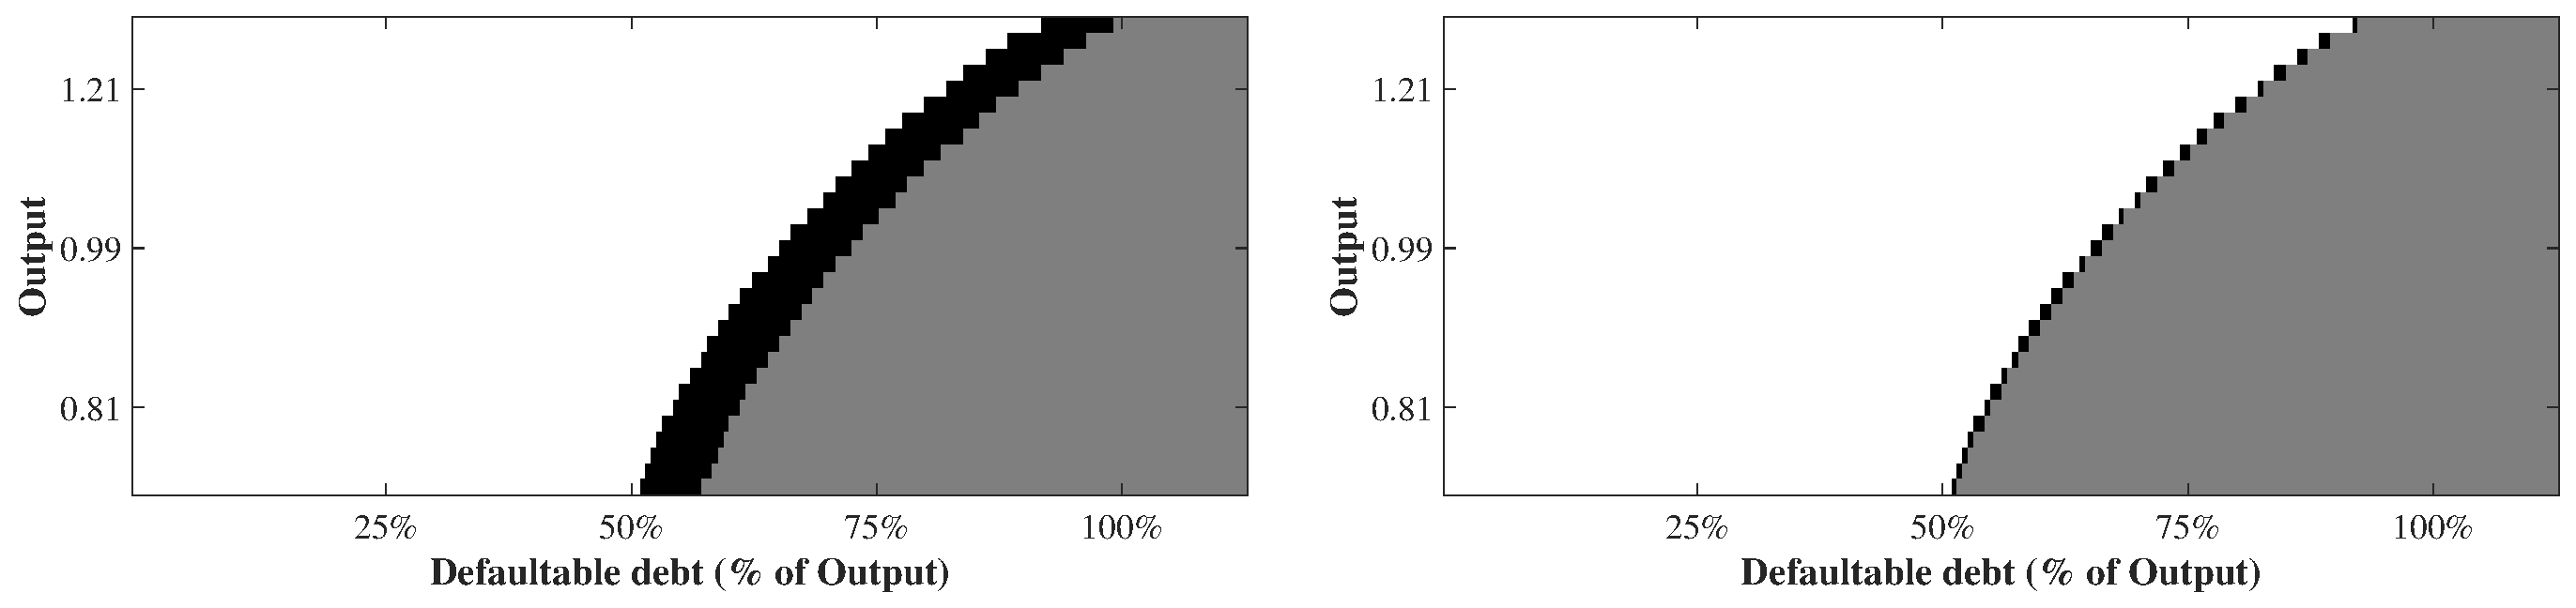
\includegraphics[scale=0.27]{default_decision_baseline.eps}
    }
    \label{fig:default decision}
        \begin{tablenotes}
      \footnotesize
    Figure 3.1 shows the default decision matrix for an economy without (black area) and an economy with Eurobonds (gray area). The left panel displays the decision where for both economies $e = 0$. The right panel shows the default decision where both economies are at their non-defaultable debt limit, $e = 0$ and $e = 0.4$ respectively.
    \end{tablenotes}
\end{figure}
%%%%%%%%%%%%%%%%%%%%%%%%%%%%%%%%%%%%%%%%%%%%%%%%%%%%%%%%%%
The first scenario (Left Panel) we take into consideration is that of two different economies: one without (black area) and one with Eurobonds where $e = 0$ (gray area). The default sets visualized for these circumstances allows us to determine if there are any combinations for defaultable debt $d$ and output $y$ for which a government would default if no Eurobonds are introduced, but would not if they are, and vice versa. As we can see, the gray area is a subset of the black area. This means that there are more combinations $(d,y)$ for which a government would default when Eurobonds are \textit{not} introduced. The reason for this difference in incentives to default can be found in the benefits of having access to non-defaultable debt. When in a state of default, there will be an exclusion period where access to the debt markets, including the one for non-defaultable debt, is limited. Non-defaultable debt can only be rolled over in a state of default and this prospect of limited market access is enough the reduce the combinations $(d,y)$ for which a government would choose to default.\\ 

The second scenario (Right Panel) portrays the default decision where both economies are considered to be at their non-defaultable debt limits, $e = 0$ (black area) and $e = 0.4$ (gray area). Similar to before, the gray area is a subset of the black area, though in a more limited way compared to the first scenario. We can therefore draw the same conclusion as the previous paragraph: default risk decreases after the introduction of Eurobonds because the potential loss of access to both the defaultable and non-defaultable debt market is enough to deter the government to default.\\

\subsubsection{Impulse response functions to introducing Eurobonds}
The second exercise illustrates the short-term effects of Eurobonds. An introduction is simulated by allowing Eurobonds to be issued at time t=0 and each period represents one quarter. Figure \ref{fig:intro} shows the average consumption, defaultable debt, risk premium and non-defaultable debt paths together with their $\pm$ two standard deviations.\\
%%%%%%%%%%%%%%%%%%%%%%%%%%%%%%%%%%%%%%%%%%%%%%%%%%%%%%%%%%
 \begin{figure}[H] 
     \centering
     \caption{\textbf{Eurobond introduction}}
     \vspace{1mm}
      \resizebox{\columnwidth}{!}{%
   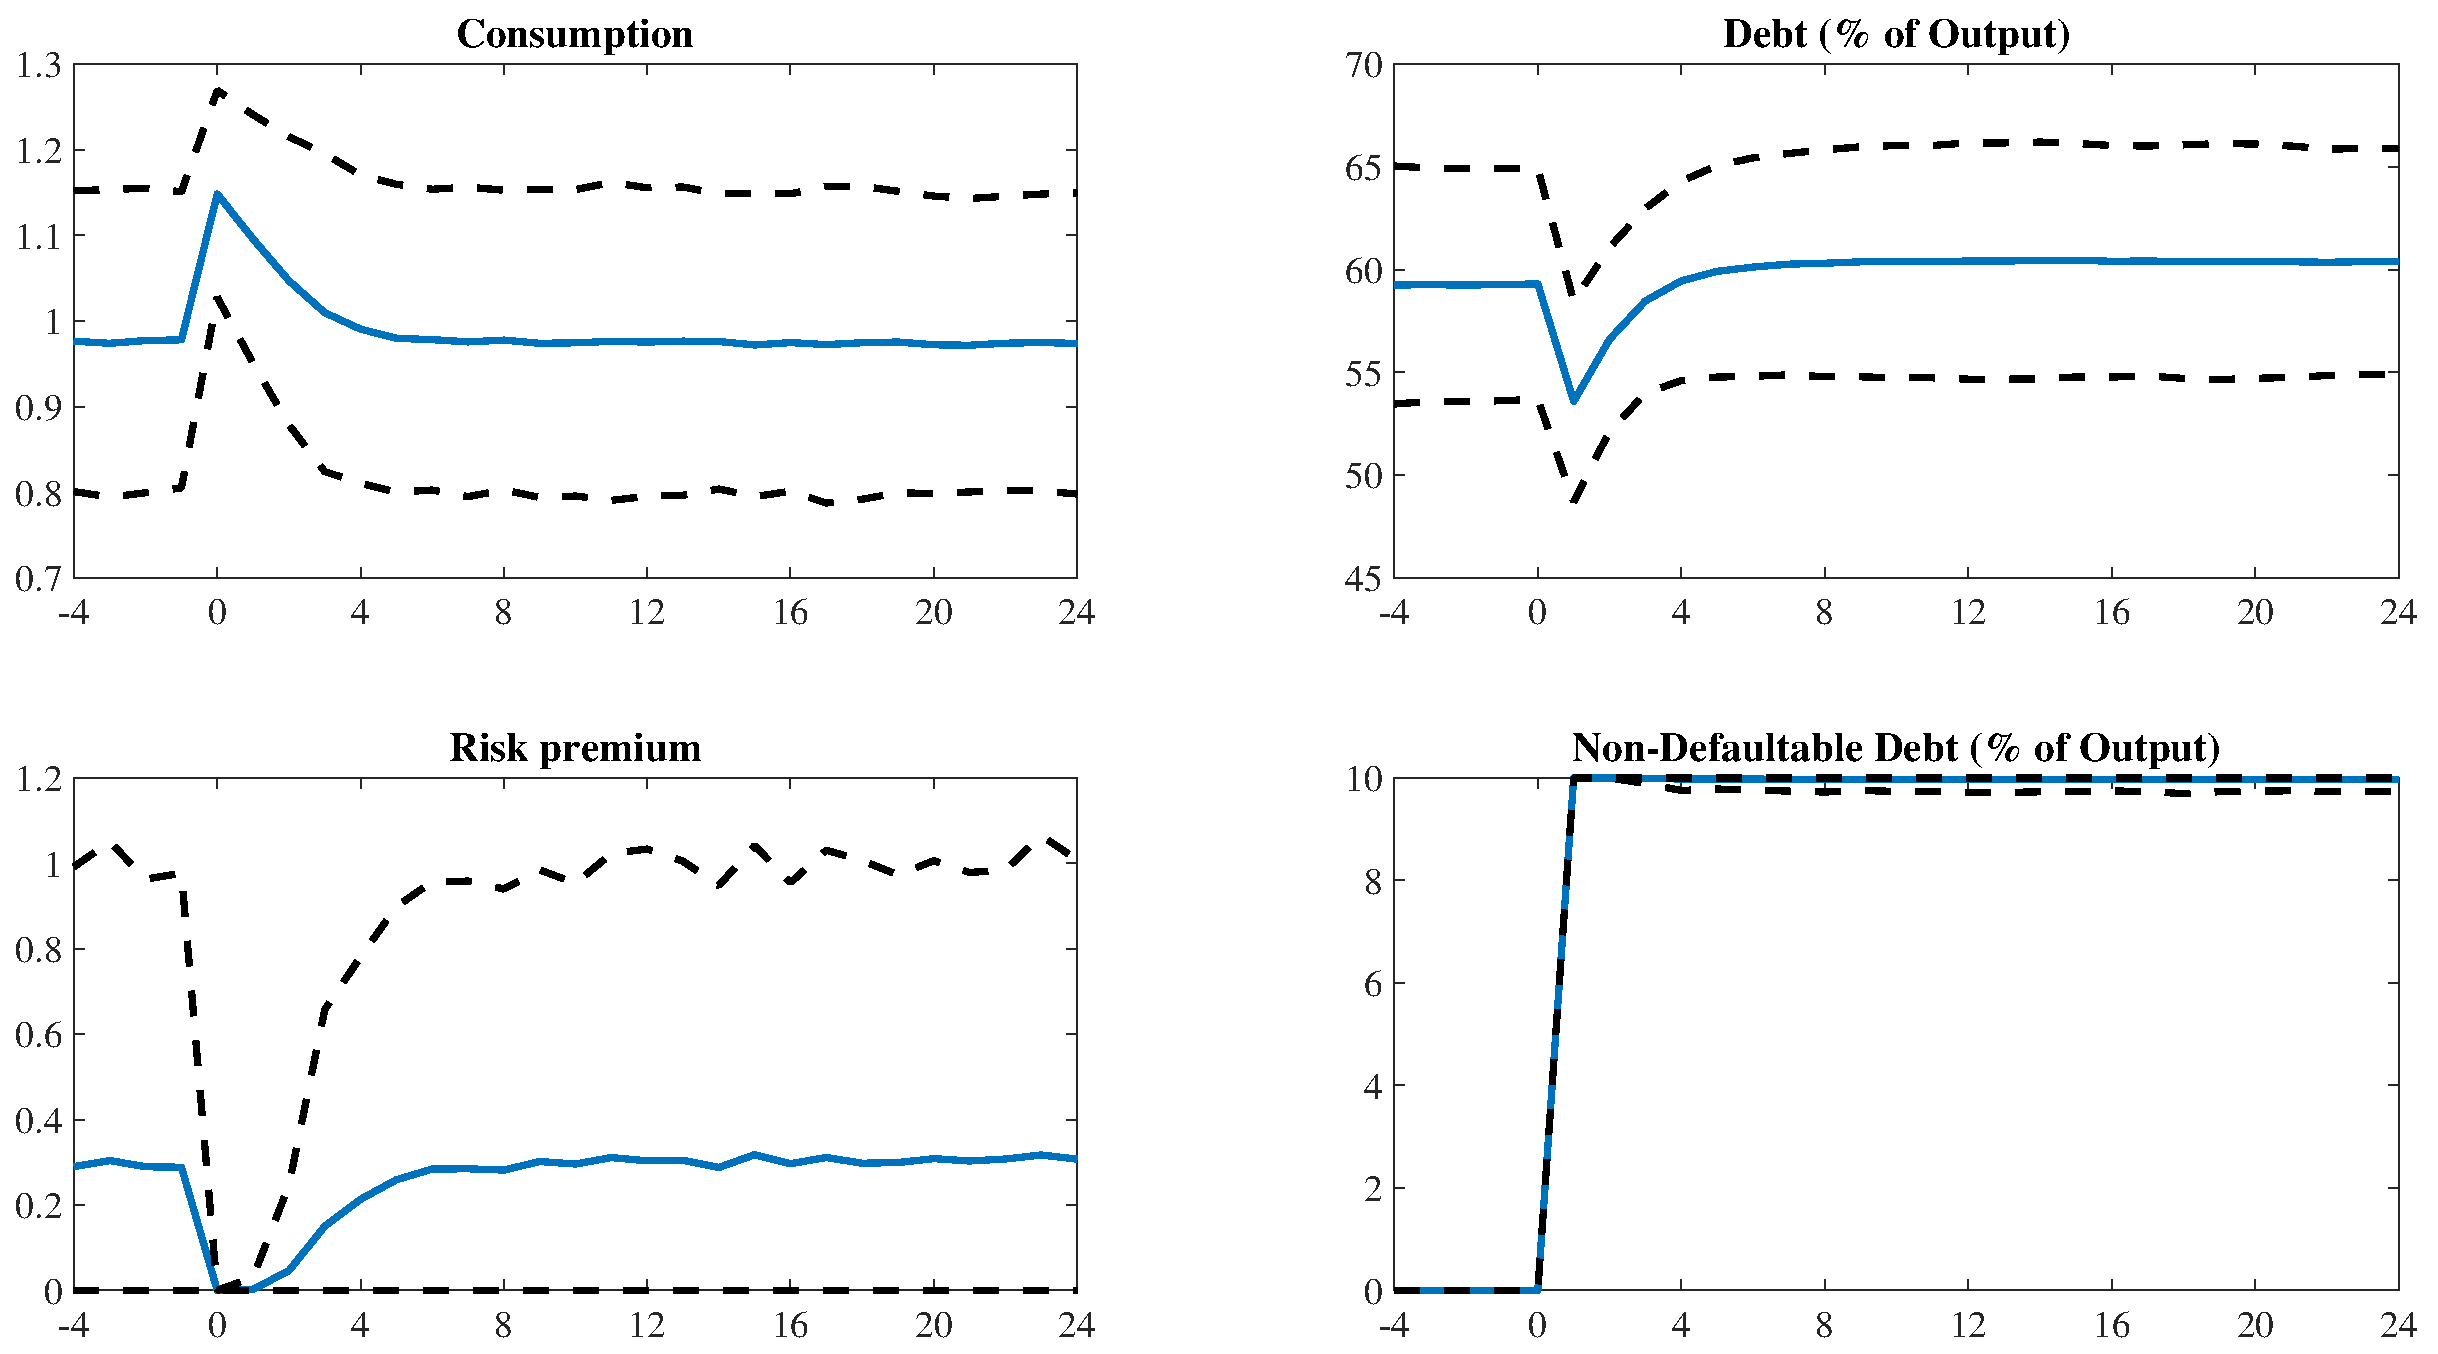
\includegraphics[scale=0.32]{Intro_baseline.eps}
    }\label{fig:intro}
      \begin{tablenotes}
      \footnotesize
      \item Figure 3.2 presents the results of an transitioning from an economy without to an economy with Eurobonds. The introduction occurs at time 0 and the response functions shown are for Consumption (Panel 1), Defaultable debt (Panel 2), the Risk Premium (Panel 3) and Non-defaultable debt (Panel 4). The full line presents the mean response and the dashed lines $\pm$ 2 standard deviations from the mean. Defaultable and non-defaultable debt are reported in \% of annual output.
      \end{tablenotes}
 \end{figure}
%%%%%%%%%%%%%%%%%%%%%%%%%%%%%%%%%%%%%%%%%%%%%%%%%%%%%%%%%%


As seen in the first panel, in the short-term there are welfare gains involved when transitioning from an economy without to one with non-defaultable debt. Consumption increases shortly after the introduction, as the government takes full advantage of the new, cheaper source of funding. On average, the non-defaultable debt limit has already been reached after one quarter. The increase in one form of debt is partially compensated by a decrease in the other. Defaultable debt decreases by roughly 7\%, which is not enough to fully compensate for the increase in its non-defaultable equivalent. This decrease in defaultable debt also lowers the average risk premium and its volatility, implying that the default risk fully disappears at the time of the introduction.\\  

As expected, however, the welfare gains of the introduction are of a short-term nature. After 4 quarters, defaultable debt and the risk premium return to their earlier levels, while non-defaultable debt remains at its limit. As any new debt needs to be repaid, the rise in consumption will also decrease over time. Nevertheless, the extra non-defaultable debt that needs to be repaid has negligible effects on consumption which will return to levels very similar to the ones before the introduction.\\ 

The analysis of the short-term effects is thus complementary to the long-term analysis. While the potential benefits of introducing a new non-defaultable form of debt are of a short-term nature, after a year the economy converges again to an equilibrium with similar defaultable debt levels, yet with a higher non-defaultable debt level. Our form of Eurobonds alone does not impose incentives to control or reduce debt levels in a model with sovereign default. In section 3.3, however, we will consider a credible debt rule which, if committed to, will play the role of a possible additional incentive to compensate for the lack of debt control in the current set-up of the model.\\
\subsection{A typical default episode}
To finalize the discussion of the baseline model, Figure \ref{fig:default_episode} presents the average default episode for an economy without and with Eurobonds. Even though the original purpose of the Eurobonds is not to mitigate default episodes, any significant changes it can have, could be useful to know in the design and policy debate. The simulations are performed for the economy with and without Eurobonds separately and the default occurs at time 0.\\
%%%%%%%%%%%%%%%%%%%%%%%%%%%%%%%%%%%%%%%%%%%%%%%%%%%%%%%%%%
\begin{figure}[H] 
     \centering
     \caption{\textbf{Typical default episode}}
     \vspace{1mm}
      \resizebox{\columnwidth}{!}{%
   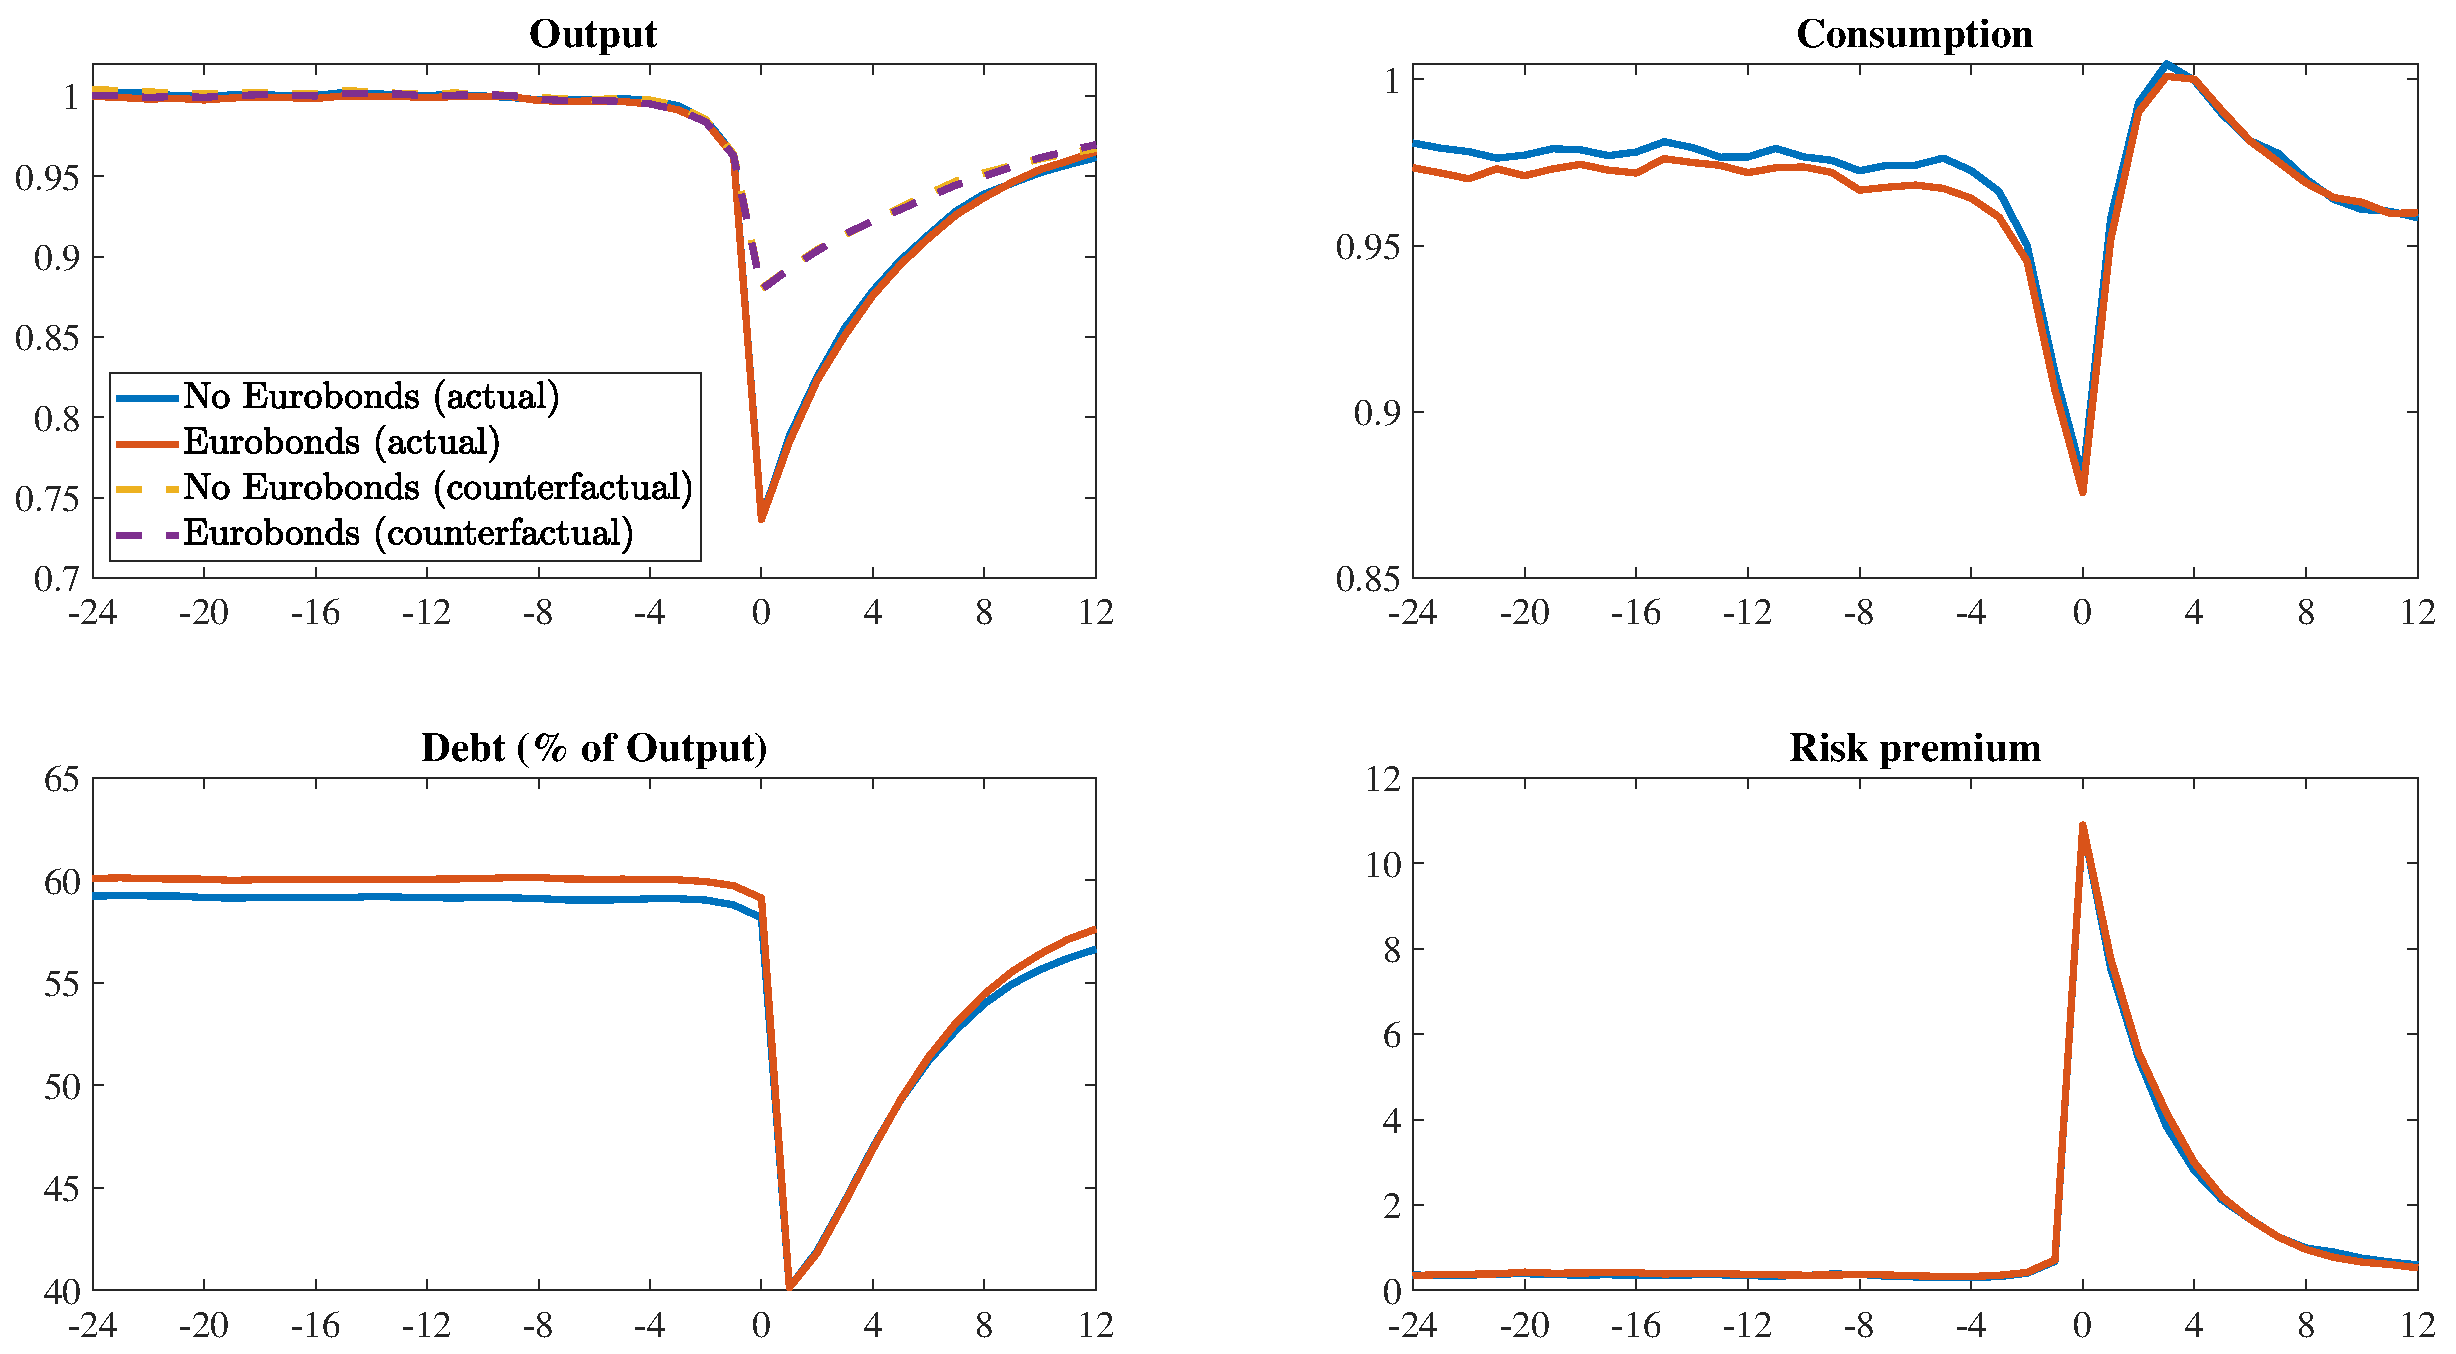
\includegraphics[scale=0.32]{typical_default_baseline.eps}
    }\label{fig:default_episode}
      \begin{tablenotes}
      \footnotesize
      \item Figure 3.4 presents the results of a typical, average default episode for an economy without (blue) and with Eurobonds (red). Average results are presented for Output, Consumption, Defaultable debt in \% of output, the Risk Premium and Non-defaultable debt in \% of output. For panel 1 the full lines present the actual output path and the dashed lines present the output path that would have been followed if no default had occurred (yellow: economy without Eurobonds, purple: economy with Eurobonds). Defaultable debt is reported in \% of annual output.
      \end{tablenotes}
    
 \end{figure}
%%%%%%%%%%%%%%%%%%%%%%%%%%%%%%%%%%%%%%%%%%%%%%%%%%%%%%%%%%
Based on the results from Figure \ref{fig:default_episode} we can make a similar conclusion to the one we made in the long-run analysis: the difference between the economy without and with Eurobonds is negligibly small. For both economies output, consumption and defaultable debt drop significantly after the default occurs, while the risk premium rises. As also shown by the dashed lines, the counterfactual output path that would have been followed had the government not decided to default also drops, though to a lesser extent than the actual path. This gap between the actual and counterfactual paths is created by the income loss $L(y)$ we assumed earlier. Overall, we can conclude our model shows no evidence Eurobonds could mitigate default episodes.\\

\section{The importance of bargaining power}
In the baseline model we assumed that the government has full control when renegotiating its debt level after a default and is committed to a self-imposed renegotiation rule $d_B = \min(d,d_S)$, similar to the model by Hatchondo et al. (2017). In practice this means that, if a default occurs, the government will offer investors a take-it-or-leave-it offer when access to the financial market is regained and investors have no way of influencing the restructured debt level. This assumption, however, may not always hold, as international power generally differs between nations and thus investor may have some influence in certain nations. This section will therefore consider a range of different values for the distribution of bargain power $\alpha$, as done in Yue (2010), and see if changing the power distribution also changes the impact of introducing Eurobonds, either in the long-run, short-run or both.\\

\subsection{Long-run impact of Eurobonds and bargaining power}
Table \ref{tab:alpha} presents the long-run statistics for different distributions of bargaining power. We will consider a range of values for $\alpha \in [0,1]$. For a complete analysis: if $\alpha = 1$ we will also consider the case where a government does not follow a specific restructuring rule and renegotiation is at its full discretion.\\

Based on the results for the different bargain schedules, three main observations can be made. First of all, regardless whether Eurobonds are introduced or not, the defaultable debt level and the default frequency increases for lower values of $\alpha$, while the risk premium and average haircut decreases. Exceptions do occur for $\alpha \in [0,0.25]$ and $\alpha = 0.45$ with Eurobonds. This, however, can be explained by the width of the grid as defaultable debt is at its limit and therefore inadequate to approximate the true solution. Nevertheless, these findings seem to conform to what Yue (2010) and Uribe \& Schmitt-Grohé (2017, p.570-571) concluded. A second observation is that following no restructuring rule ($\alpha = 1$) has a significant impact on how much debt can be supported in equilibrium. With no rule, the average haircut is near 100\% which implies a lot more risk is involved for investors who will adjust their debt pricing accordingly. The third and most important observation is that with the introduction of Eurobonds, defaultable debt levels drastically increase for any $\alpha \neq 1$, though not in a monotonic fashion. In addition, the risk premia are also lower in the economy with Eurobonds, hinting at overall lower risk. The reason as to why this occurs has to do with the influence investors have in renegotiation which we will cover in section 3.2.3.\\
\subsection{Short-run effects of Eurobonds and bargaining power}
Similar to the baseline results, to see the short-run impact of introducing Eurobonds in different bargaining schedules the average impulse response functions of consumption, defaultable debt, the risk premium and non-defaultable debt are visualized in Figure \ref{fig:intro_comp}. We will only consider the cases of $\alpha \in [0.55,1]$ as these give us the most reliable results (cf. Table \ref{tab:alpha}).\\
%%%%%%%%%%%%%%%%%%%%%%%%%%%%%%%%%%%%%%%%%%%%%%%%%%%%%%%%%%
\begin{table}[H]\Large
\setlength{\arrayrulewidth}{0.3mm}
\centering
    \caption{\textbf{Model statistics for different distributions of bargaining power $\alpha$}}
    \label{tab:alpha}
    \vspace{1mm}
   \resizebox{\columnwidth}{!}{%
 \begin{tabular}{lm{2.6cm}cccccc} 
\hline\hline
\textbf {Model}                 &  \textbf {Default frequency}       &$\bm{E(\frac{d}{Y})}$& $\bm{E(\frac{e}{Y})}$&  $\bm{E(r-r^*)}$& $\bm{\sigma(r-r^*)}$ & $\bm{corr(r-r^*,y)}$& $\bm{E(h)}$           \\
\hline\hline
\textit{\underline{Baseline}}  &    &      &     &     &      &  & \\[1ex] 
\textit{\bm{$\alpha = 1 \text{ } \|\text{ } d_B \text{ \textbf{rule} (No Eurobonds)}$}}  & 0.8436    & 59.21     & 0     & 0.2852    & 0.342     & -0.4236   & 30.85 \\[1ex] 
\textit{\bm{$\alpha = 1 \text{ } \|\text{ } d_B \text{ \textbf{rule} (Eurobonds)}$}}  &0.8428     & 60.21     & 9.99  & 0.3034    & 0.3502    &-0.4517    & 32          \\[1ex] 
\textit{\underline{Alternative values for $\alpha$ (No Eurobonds)}}  &    &      &     &     &      &  & \\[1ex] 
\textit{\bm{$\alpha = 0.00 $}}  &  n.a.   &  112.79    &   0 & n.a. & n.a.  &  n.a. & n.a. \\[1ex]                                 
\textit{\bm{$\alpha = 0.25 $}}  &  n.a.   &   112.88   &   0   &    n.a. & n.a.   &  n.a. & n.a.  \\[1ex]                                 
\textit{\bm{$\alpha = 0.45$}}  & 1.9732    &  98.18    &   0   &  0.3613   &  0.4885    & -0.4818  & 13.96 \\[1ex]
\textit{\bm{$\alpha = 0.55$}}  & 1.714    & 79.26  & 0  &  0.395    &  0.5307   &   -0.4928   &   19.29  \\[1ex]
\textit{\bm{$\alpha = 0.65$}} &1.5656 &  63.36   &  0    & 0.4866     & 0.6651    &  -0.4898    &   26.63  \\[1ex]
\textit{\bm{$\alpha = 0.75$}}  &  1.2836   &   49.52   &  0    &  0.5434   &    0.7248  & -0.489  & 36.84 \\[1ex]
\textit{\bm{$\alpha = 1.00 \text{ } \| \text{\textbf{ no }} d_B \text{\textbf{ rule}}$}}  & 0.7912    & 22.21     & 0     & 0.8671    & 1.0413     & -0.4862   & 99.99\\[1ex] 
\textit{\underline{Alternative values for $\alpha$ (Eurobonds)}}  &    &      &     &     &      &  & \\[1ex]
\textit{\bm{$\alpha = 0.00$}}  &  n.a. & 112.83  & 10.03     &    n.a. & n.a.   &   n.a. & n.a.  \\[1ex]  
\textit{\bm{$\alpha = 0.25$}}  &   n.a. & 112.77  &10.02    &      n.a. & n.a.     & n.a. & n.a. \\[1ex] 
\textit{\bm{$\alpha = 0.45$}}  & 0.3468 & 112.53  & 10.02  &  0.0481  &  0.1630 &  -0.5256 & 9.66  \\[1ex] 
\textit{\bm{$\alpha = 0.55$}}  &  1.7072 &  95.75  &  9.96   & 0.3239 &   0.4354 &  -0.4997 & 15.33  \\[1ex]
\textit{\bm{$\alpha = 0.65$}}  &  1.5576  & 75.29 &   9.98  &  0.4103  &  0.5535 &  -0.4933 &  22.04\\[1ex]
\textit{\bm{$\alpha = 0.75$}}  &   1.2880  & 57.54 &9.92  &  0.4678   & 0.6245  & -0.4772  &  31.78\\[1ex]
\textit{\bm{$\alpha = 1.00 \text{ } \| \text{\textbf{ no }} d_B \text{\textbf{ rule}}$}}  & 0.7300 &  23.63  &  9.90    &0.7479   & 0.8979  & -0.4553 & 97.47          \\[1ex]     
\hline\hline
\end{tabular}}
    \begin{tablenotes}
      \footnotesize
      \item Model statistics are calculated under the condition a country finds itself in good standing. The default frequency is reported on an annual basis. The symbols E, $\sigma$ and corr represent the average, standard deviation and correlation. Average defaultable $E(\frac{d}{Y})$ and non-defaultable debt $E(\frac{e}{Y})$ are reported in \% of annual output $Y = 4y$. The Risk Premium and haircut are presented as $r-r^*$ and $h$, respectively. The special case $\alpha = 1$ is calculated once with (baseline) and once without the special rule for $d_B$ (alternative).
    \end{tablenotes}
\end{table}
%%%%%%%%%%%%%%%%%%%%%%%%%%%%%%%%%%%%%%%%%%%%%%%%%%%%%%%%%%


While we find that for all values of $\alpha$ there are welfare gains of introducing Eurobonds, the intensity of these gains varies between the different economies. The economies where investors have more influence in the restructuring process ($\alpha = \{0.55,0.65,0.75\}$) lead to a significantly higher increase in consumption compared to the economy where they have no influence. This can partially be explained by the lower initial buyback or decrease in defaultable debt for lower values of $\alpha$. This combined with the relatively higher decrease in risk premia and increase in non-defaultable debt leads to a higher and longer increase in consumption as consumption returns to its original level only after 8 quarters compared to 4 quarters in the baseline model.  Nonetheless, the most notable difference seems once more to occur in medium- to long-run convergence of the defaultable debt level. For all economies with $\alpha \neq 1$ the defaultable debt level converges to a higher level than before the introduction, implying the influence of investors is non-trivial.\\
%%%%%%%%%%%%%%%%%%%%%%%%%%%%%%%%%%%%%%%%%%%%%%%%%%%%%%%%%%
 \begin{figure}[H]
\caption{\textbf{Introducing the Eurobond in different bargaining schedules}}
    \centering
    \vspace{1mm}
     \resizebox{\columnwidth}{!}{%
   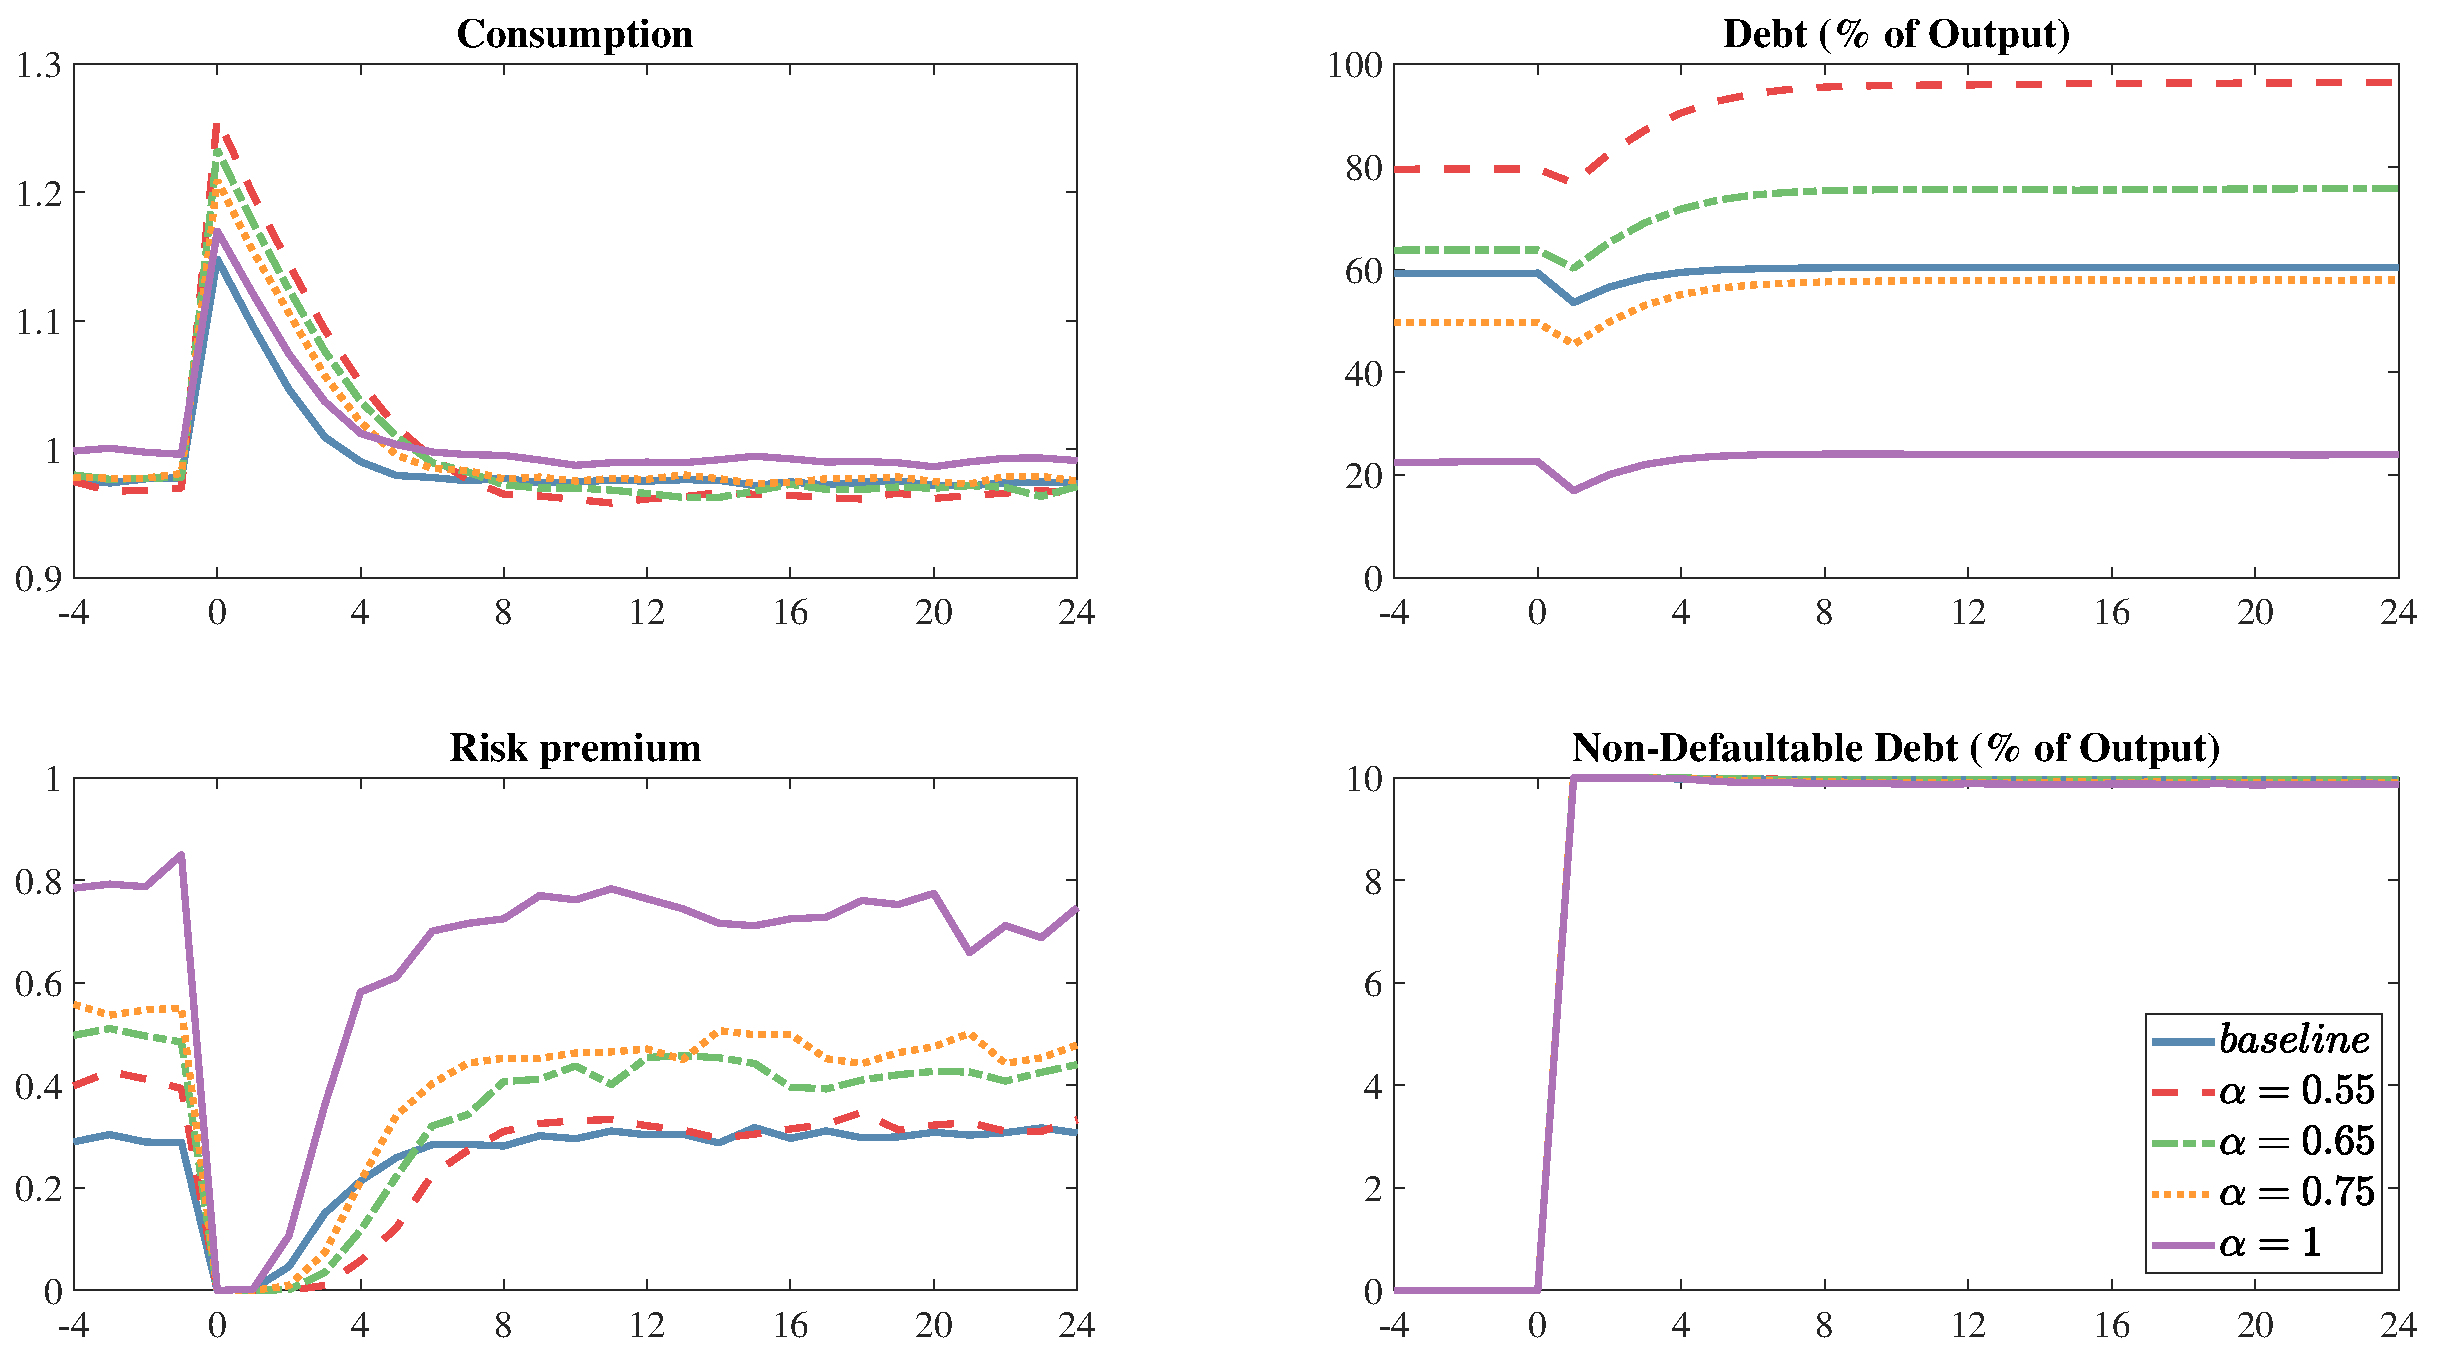
\includegraphics[scale=0.28]{Intro_comp.eps}
    }
    \label{fig:intro_comp}
        \begin{tablenotes}
      \footnotesize
   Figure 3.4 presents the results of transitioning from an economy without to an economy with Eurobonds for the baseline model and different values for $\alpha$. The introduction occurs at time 0 and the average response functions are shown for Consumption (Panel 1), Defaultable debt (Panel 2), the Risk Premium (Panel 3) and Non-defaultable debt (Panel 4). Defaultable and non-defaultable debt are reported in \% of annual output.
    \end{tablenotes}
\end{figure}
%%%%%%%%%%%%%%%%%%%%%%%%%%%%%%%%%%%%%%%%%%%%%%%%%%%%%%%%%%
\subsection{The influence of investors after the introduction of Eurobonds}
Both the long-run and short-run analysis show that the bargain power distribution has a significant impact on the long-run debt level when Eurobonds are introduced. This impact is most apparent for $\alpha \in [0.55,0.75]$. To explain these differences, we will distinguish two phases in which the role of investors affect the debt incentive structure: the renegotiation phase and a "Price \& Debt adjustment" phase.\\

 In the renegotiation phase, there is a distinction between $\alpha = 1$ and $\alpha \neq 1$. If $\alpha = 1$ the government has full control and its optimal strategy will not change, regardless if it has access to Eurobonds or not. If $\alpha \neq 1$, however, investors will be involved in the renegotiation process and a compromise needs to be found between the two interest groups. Recall that the surplus of the investors is determined by $q_B(d_B,e,y)d_B$ and that the default risk decreases for some combinations of $(d,y)$ as shown by Figure \ref{fig:default decision} (complemented by Figures A.1-A.4 in Appendix A). This suggests that, as soon as Eurobonds are introduced, default risk decreases for certain combinations of $(d,y)$ which results in a higher price $q$ and $q_B$ for debt in this region. Because of this higher price, creditors will also gain a larger surplus if they readjust their bargain position, particularly for those combinations of $(d,y)$ that were considered to be risky before, yet not anymore. With the readjustment in the bargain position of investors and an unchanged strategy for the government, the result of the renegotiation is a higher recovery rate $\frac{d_B(y)}{d}$ after default, which explains the lower haircut after the introduction of Eurobonds.\\ 
 
 This renegotiation phase is then followed by a "Price \& Debt adjustment" phase. As the recovery rate increases after the introduction of Eurobonds, investors will once more readjust the pricing of debt contracts. After all, the recovery rate is part of the price equations \eqref{ZP not default} and \eqref{ZP default}. With a higher recovery rate investors will lose less if a default occurs, therefore prices of debt will go up as there is less risk involved. From the government's point of view higher prices for debt imply lower costs of borrowing, making borrowing more attractive. The government will thus take advantage of this reduction in costs and seek to increase its borrowing level.\\
 
What results out of the two phases is what we observe both in Table \ref{tab:alpha} and Figure \ref{fig:intro_comp}: the frequency of defaults stays relatively the same after the introduction of Eurobonds, while debt levels, both defaultable and non-defaultable, increase more if investors can exert more influence on the renegotiation process. The policy implication that follows from this extension is that disregarding the balance of power can affect the overall evaluation of Eurobonds. Nations with different bargain power may experience different changes in incentive structures. Without any additional debt control incentives debt levels can rise significantly, especially for those nations where investors are able to influence the restructuring process.\\

\section{Potential benefit of a credible debt rule}
As a last addition to our analysis we will simulate the effects of introducing Eurobonds together with a credible debt rule. Considering that Eurobonds do not incentivise governments to reduce debt, additional fiscal rules may need to be imposed to guarantee compliance with the fiscal framework of the European Union. As argued by Hatchondo et al. (2017) introducing Eurobonds could also potentially help in financing this transition to specific fiscal rules or targets. The question then remains: do Eurobonds still provide benefits if introduced with additional fiscal rules?\\

Figure \ref{fig:intro_debtrule} shows the result of introducing Eurobonds together with a debt rule. In combination with the announcement of Eurobonds, the government announces that a new debt rule of a defaultable debt-to-GDP ratio of 50\% will be imposed. We will not go into detail on how it is implemented and we simply assume it to be a rule to which the government is able to commit. The limit of defaultable debt to 50\% is chosen such that it reduces all risk of default and is conform to the Maastricht criteria of 60\% debt-to-GDP when summed up with the non-defaultable debt limit (European Commission, 2019).\\

Despite the limitation on defaultable debt, introducing Eurobonds still delivers benefits to welfare in the short-run. All economies\footnote{Note that $\alpha = 1$ without a $d_B$ rule is left out of Figure \ref{fig:intro_debtrule}, since introducing a debt rule of 50\% would have no effect on this parameterisation of the model.} experience an increase in consumption and a reduction in defaultable debt and risk premia. Unlike the scenario without a debt rule, however, the increase in consumption is more short-lived for the economies with lower $\alpha$'s. Nonetheless, the commitment to the debt rule reduces defaultable debt in the long-run to the extent that all default risk disappears and borrowing is done at the risk-free rate.\\
%%%%%%%%%%%%%%%%%%%%%%%%%%%%%%%%%%%%%%%%%%%%%%%%%%%%%%%%%%
 \begin{figure}[H]
\caption{\textbf{Introducing the Eurobond in different bargaining schedules together with a debt rule}}
    \centering
    \vspace{1mm}
     \resizebox{\columnwidth}{!}{%
   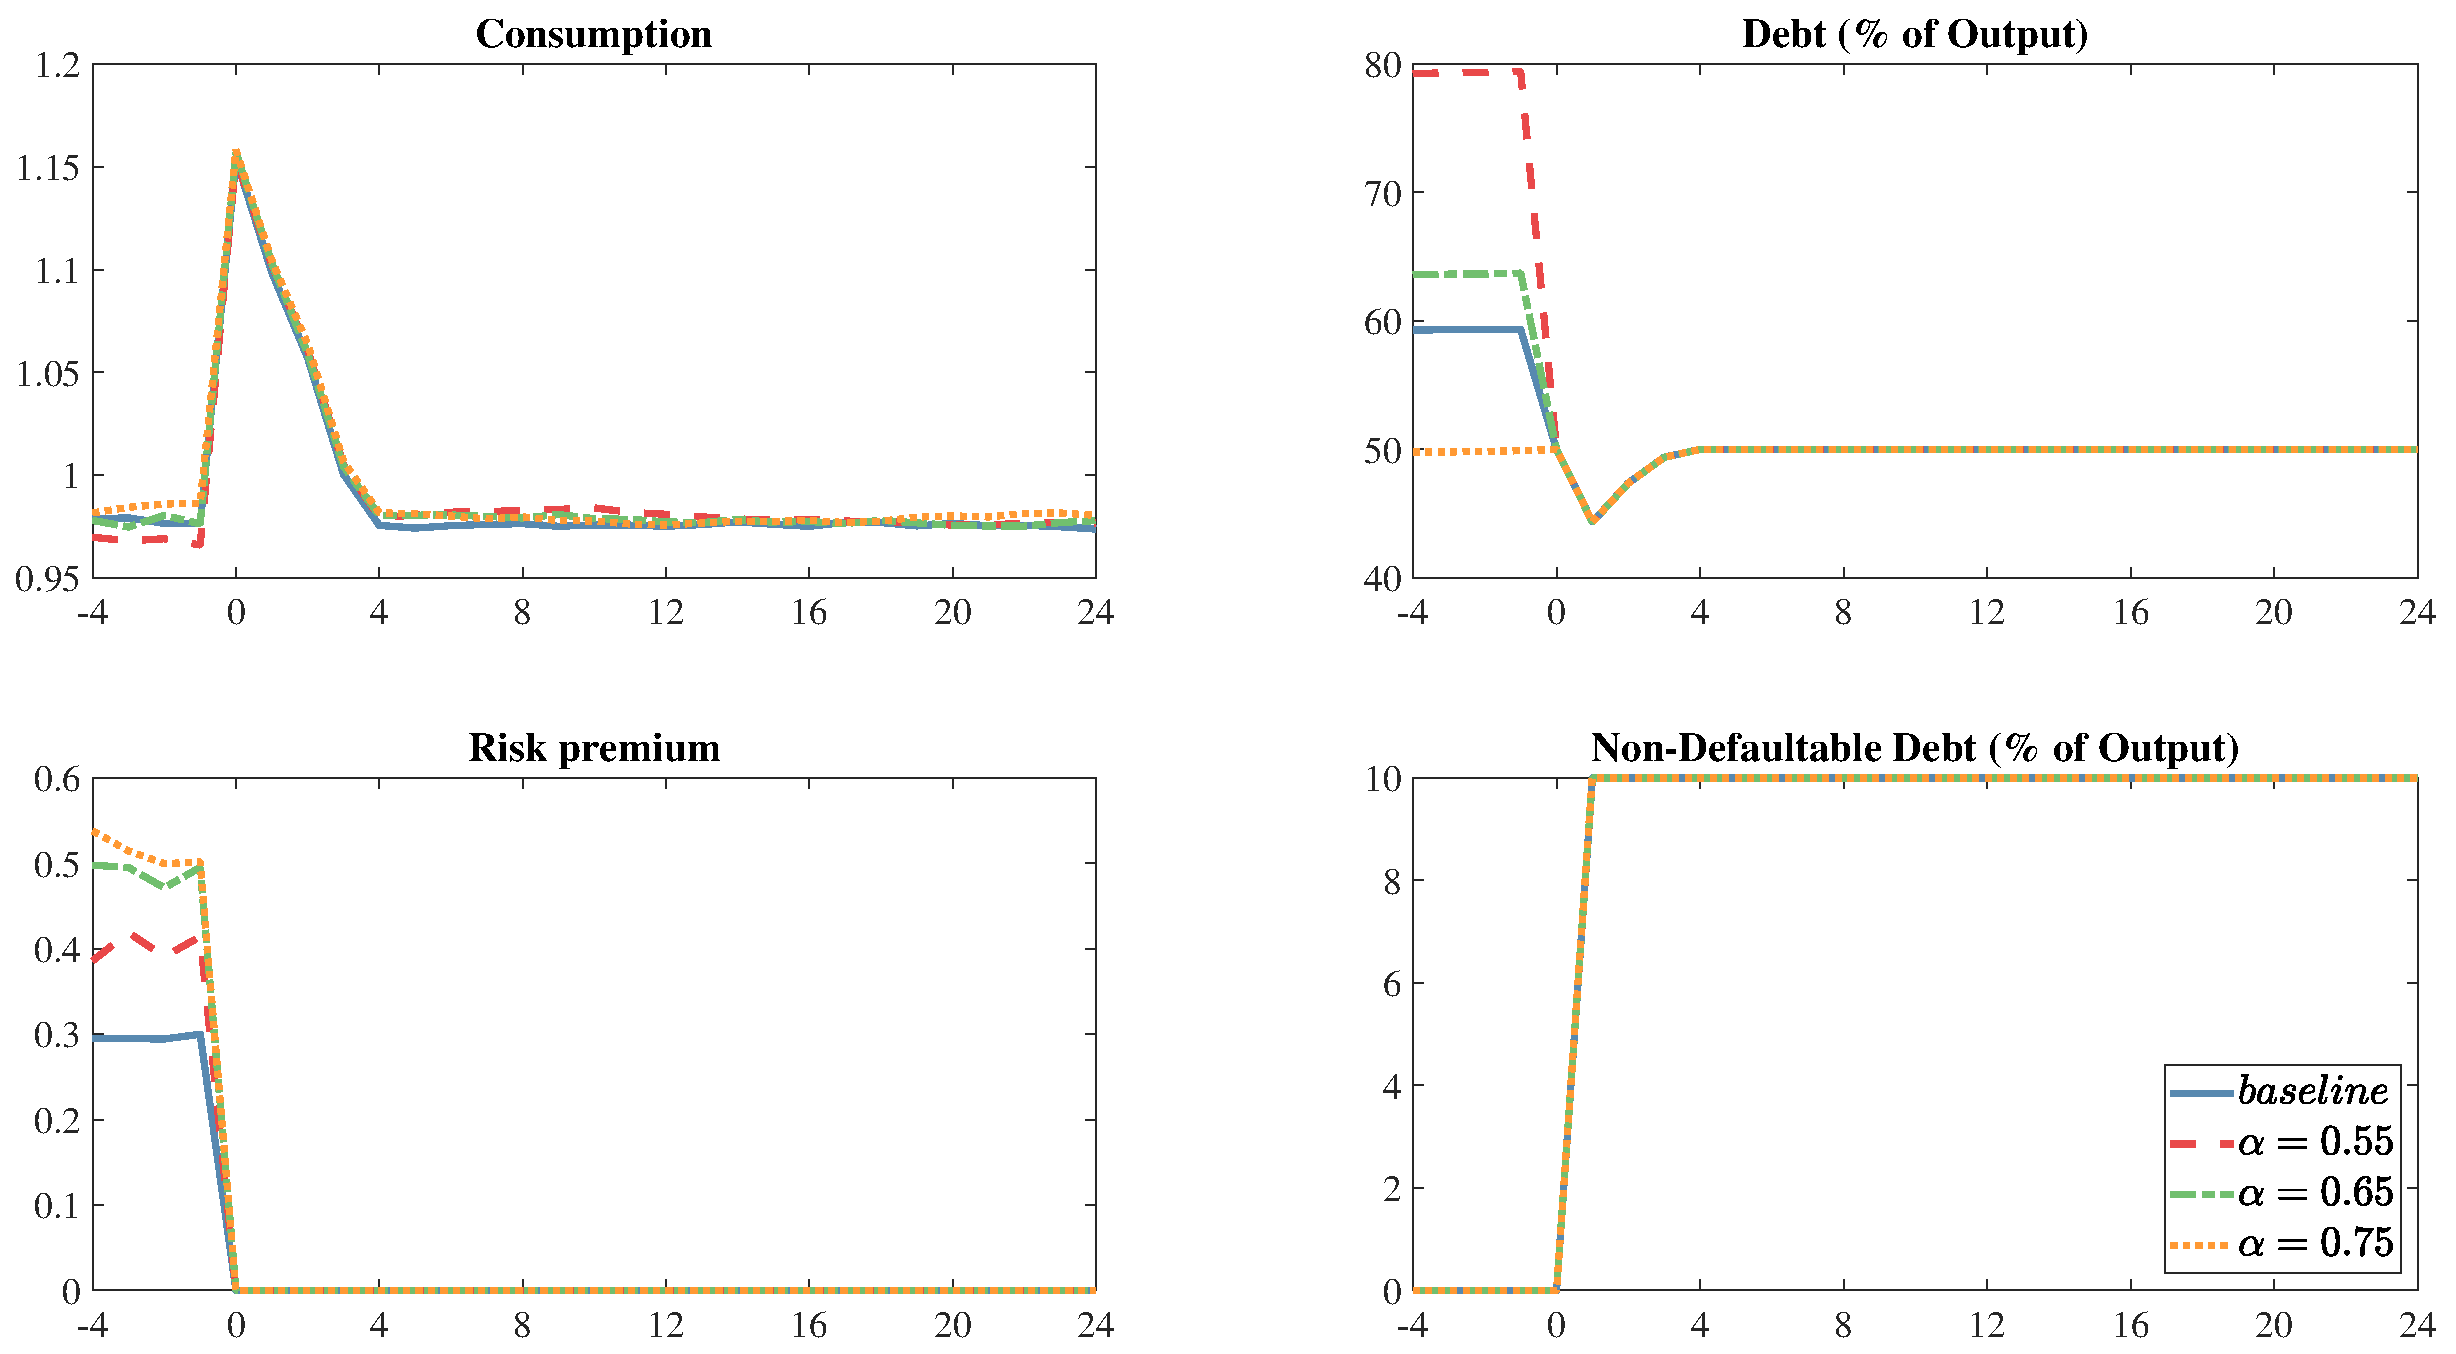
\includegraphics[scale=0.28]{Intro_debtrule.eps}
    }
    \label{fig:intro_debtrule}
        \begin{tablenotes}
      \footnotesize
   Figure 3.5 presents the results of transitioning from an economy without to an economy with Eurobonds for the baseline model and different values for $\alpha$ in addition to a debt rule. The introduction occurs at time 0 and the average response functions shown are for Consumption (Panel 1), Defaultable debt (Panel 2), the Risk Premium (Panel 3) and Non-defaultable debt (Panel 4). Defaultable and non-defaultable debt are reported in \% of annual output. To ensure compatibility of the two calibrated models and their policy functions, the number of grid points for Defaultable Debt nd is lowered to 100 in the economy with the debt rule.
    \end{tablenotes}
\end{figure}
%%%%%%%%%%%%%%%%%%%%%%%%%%%%%%%%%%%%%%%%%%%%%%%%%%%%%%%%%%
\section{Robustness of the model}
As a final step in our analysis, we will perform a robustness check of the baseline model. Four specific tests to the robustness of our results will be considered: the sensitivity to alternatives of the exclusion duration $\theta$, the sensitivity to the non-defaultable debt limit, the sensitivity to the grid specification and, lastly, the possible occurrence of multiple equilibria.\\
\subsection{Sensitivity to the duration of the exclusion period}
In the baseline model it is assumed that once a default occurs, access to financial markets is regained within the year (3.5 quarters for $\theta = 0.282$). The use of this calibrated value conforms to estimates by Gelos et al. (2004) and is used by several papers in the sovereign default literature (e.g. Hatchondo et al., 2017; Önder \& Sunel,  2020). However, Gelos et al.'s estimates are based on a data-set of developing economies and a revision of their earlier work re-estimates an average exclusion of 2.9 years based on data from the 1990s (Gelos, Sahay \& Sandleris, 2011). As our model is calibrated to a European economy, we consider a more prudent stance and test the sensitivity of the results to different probabilities of reentry $\theta$.\\
\clearpage
To account for some possible uncertainty we will re-calibrate the baseline model to a lower and higher value for $\theta$ and see how this affects the results. The higher value is a fictional value of 0.5 which implies a shorter, average reentry within 2 quarters. The lower value we calibrate to the findings of Guscina, Malik \& Papaioannou (2017) who estimate an average exclusion period of 19 months ($\theta = 0.210$) between the period of 2010-2015 for a data-set of both developing and developed countries.\\

Table \ref{tab:theta} shows the results for the different calibrations of $\theta$. Conform to the expectations, a lower $\theta$ corresponds to a lower default frequency. A longer exclusion period makes defaulting less attractive as access to financial markets is lost for a longer period of time. With these lower default incentives, investors will price bonds higher which in turn allows for a higher debt level. The opposite interactions can be observed when $\theta$ is higher. That being said, different values of $\theta$ do not seem to alter our conclusion on Eurobonds from the baseline model. Both economies behave similarly in the long-run and any differences are negligibly small.\\
%%%%%%%%%%%%%%%%%%%%%%%%%%%%%%%%%%%%%%%%%%%%%%%%%%%%%%%%%%
\begin{table}[H]\Large
\setlength{\arrayrulewidth}{0.3mm}
\centering
    \caption{\textbf{Model statistics for different reentry probabilities $\theta$}}
    \label{tab:theta}
    \vspace{1mm}
   \resizebox{\columnwidth}{!}{%
 \begin{tabular}{lm{2.1cm}cccccc} 
\hline\hline
\textbf {Model}                 &  \textbf {Default frequency}       &$\bm{E(\frac{d}{Y})}$& $\bm{E(\frac{e}{Y})}$&  $\bm{E(r-r^*)}$& $\bm{\sigma(r-r^*)}$ & $\bm{corr(r-r^*,y)}$& $\bm{E(h)}$           \\
\hline\hline
\textit{\underline{Baseline}}  &    &      &     &     &      &  & \\[1ex] 
\textit{\bm{$\theta = 0.282 \text{ (No Eurobonds)}$}}  & 0.8436    & 59.21     & 0     & 0.2852    & 0.342     & -0.4236   & 30.85 \\[1ex] 
\textit{\bm{$\theta = 0.282 \text{ (Eurobonds)}$}}   &0.8428     & 60.21     & 9.99  & 0.3034    & 0.3502    &-0.4517    & 32          \\[1ex]   
\textit{\underline{Alternative values for $\theta$}}  &    &      &     &     &      &  & \\[1ex] 
\textit{\bm{$\theta = 0.210 \text{ (No Eurobonds)}$}}  &  0.6512  & 66.33  &      0  &  0.2847  &  0.3759  & -0.4170 & 38.36\\[1ex] 
\textit{\bm{$\theta = 0.210 \text{ (Eurobonds)}$}}  &  0.6904  & 68.15  &  9.52 &   0.3165 &   0.3720 &  -0.4234 & 40.23        \\[1ex]
\textit{\bm{$\theta = 0.500 \text{ (No Eurobonds)}$}}  & 1.1480  & 50.59  &      0 &   0.2528  &  0.2508  & -0.3567  & 19.56\\[1ex] 
\textit{\bm{$\theta = 0.500 \text{ (Eurobonds)}$}}  &    1.0828 &  51.15  & 9.99  &  0.2504  &  0.2366  & -0.4359   &     20.27   \\[1ex]     \hline\hline
\end{tabular}}    
\begin{tablenotes}
      \footnotesize
      \item Model statistics are calculated under the condition a country finds itself in good standing. The default frequency is reported on an annual basis. The symbols E, $\sigma$ and corr represent the average, standard deviation and correlation. Average defaultable $E(\frac{d}{Y})$ and non-defaultable debt $E(\frac{e}{Y})$ are reported in \% of annual output $Y = 4y$. The risk premium and haircut are presented as $r-r^*$ and $h$, respectively.
    \end{tablenotes}
\end{table}
%%%%%%%%%%%%%%%%%%%%%%%%%%%%%%%%%%%%%%%%%%%%%%%%%%%%%%%%%%
\subsection{Sensitivity to the non-defaultable debt limit}
Similar to the analysis performed by Hatchondo et al. (2017) we assumed that the non-defaultable debt limit was set at 10\% of GDP. Setting this limit makes our analysis comparable to Philippon \& Hellwig's Eurobill proposal (2011). Other proposals, for example the Blue-Red bond proposal by Delpla \& Von Weizsäcker (2010) or the Redemption Pact (Doluca et al., 2012), suggest a larger percentage of debt to be mutualised. The model can be easily adjusted to account for these larger Eurobond limits by increasing the upper limit $\bar{e}_R$. We will perform a smaller adjustment of up to 20\% and a larger change of up to 60\% to test the sensitivity of our results. A drawback of extending the upper limit, however, is that by doing so we also increase the coarseness of the grid if we do not also increase the number of grid points. The discussion on the importance of the grid specification is left for section 3.4.3.\\ 
%%%%%%%%%%%%%%%%%%%%%%%%%%%%%%%%%%%%%%%%%%%%%%%%%%%%%%%%%%
\begin{table}[H]\large
\setlength{\arrayrulewidth}{0.3mm}
\centering
    \caption{\textbf{Sensitivity of results to the non-defaultable debt limit}}
    \label{tab:non-defaultable debt limit}
    \vspace{1mm}
   \resizebox{\columnwidth}{!}{%
 \begin{tabular}{lm{2.5cm}cccccc} 
\hline\hline
\textbf {Model}                 &  \textbf {Default frequency}       &$\bm{E(\frac{d}{Y})}$& $\bm{E(\frac{e}{Y})}$&  $\bm{E(r-r^*)}$& $\bm{\sigma(r-r^*)}$ & $\bm{corr(r-r^*,y)}$& $\bm{E(h)}$           \\
\hline\hline
\textit{\bm{$\bar{e}_R = 0.4$}}     &0.8428     & 60.21     & 9.99  & 0.3034    & 0.3502    &-0.4517    & 32          \\[1ex]    
\textit{\bm{$\bar{e}_R = 0.8$}}     &0.7412&   60.89 & 20.04 &   0.2745  &  0.3256  & -0.3953 & 32.95\\[1ex]
\textit{\bm{$\bar{e}_R = 2.4$}}     &0.7692 &  64.11 &  60.16  &  0.3047 &   0.3549  & -0.4157 & 36.29 \\[1ex]      
\hline\hline             
\end{tabular}}
    \begin{tablenotes}
      \footnotesize
      \item Model statistics are calculated under the condition a country finds itself in good standing. The default frequency is reported on an annual basis. The symbols E, $\sigma$ and corr represent the average, standard deviation and correlation. Average defaultable $E(\frac{d}{Y})$ and non-defaultable debt $E(\frac{e}{Y})$ are reported in \% of annual output $Y = 4y$. The risk premium and haircut are presented as $r-r^*$ and $h$, respectively.
    \end{tablenotes}
\end{table}
%%%%%%%%%%%%%%%%%%%%%%%%%%%%%%%%%%%%%%%%%%%%%%%%%%%%%%%%%%
Table \ref{tab:non-defaultable debt limit} shows that altering the non-defaultable debt limit has no large impact on the model performance, other than increasing the average non-defaultable debt-to-GDP ratio. Both economies with $\bar{e}_R = 0.8$ and $\bar{e}_R = 2.4$ will stay at their Eurobond limit in the long-run and there are no incentives to decrease defaultable debt, similar to the results of the baseline model.\\
\subsection{Sensitivity to the grid specification}
Hatchondo, Martinez \& Sapriza (2010) caution in their paper on numerical solution methods of sovereign default models that using Discrete State Space approaches with an insufficient amount of grid points can lead to spurious interest rate movements and unreliable results. Uribe \& Schmitt-Grohé (2017, p.530-533) also support this critique by showing that increasing or decreasing the endowment grid can alter the results of the model. To test for possible misspecification, we consider 9 alternative grids for our model. In our analysis, however, we limited the number of possible elements of a grid to 120.000 as working with larger grids often led to memory issues or extremely long computation times in \texttt{Matlab}.\\

Table \ref{tab:grid} lists the results for our different grid specifications. To study the sensitivity we perform four categories of alterations: i) a variation of different non-defaultable debt points $ne$, ii) a variation of different defaultable debt points $nd$, iii) a variation of both defaultable and non-defaultable points $(nd,ne)$ and iv) a variation of output points $ny$.\\

The results of Table \ref{tab:grid} show that while the predictions do not deviate much of one another, some caution is warranted. Estimates for the default frequency range from 0.704 to 0.9292, which corresponds to a default every 142 to 108 years. Furthermore, even as defaultable debt stays around 60\%, its non-defaultable counterpart seems to be sensitive to changes in both the defaultable and non-defaultable debt grid. Both for a lower amount of grid points $nd$ and higher amount for $ne$ does the average debt ratio for Eurobonds decrease, from 9.99\% in the baseline to 7.8\% in the grid (30,20,200). This implies that our earlier finding that non-defaultable debt is almost always at its limit may be a result of our chosen grid and thus not entirely accurate for all grid approximations.\\
%%%%%%%%%%%%%%%%%%%%%%%%%%%%%%%%%%%%%%%%%%%%%%%%%%%%%%%%%%
\begin{table}[H]\Large
\setlength{\arrayrulewidth}{0.3mm}
\centering
    \caption{\textbf{Model statistics for different grid specifications}}
    \label{tab:grid}
    \vspace{1mm}
   \resizebox{\columnwidth}{!}{%
 \begin{tabular}{lm{2.6cm}cccccc} 
\hline\hline
\textbf {Grid size}                 &  \textbf {Default frequency}       &$\bm{E(\frac{d}{Y})}$& $\bm{E(\frac{e}{Y})}$&  $\bm{E(r-r^*)}$& $\bm{\sigma(r-r^*)}$ & $\bm{corr(r-r^*,y)}$& $\bm{E(h)}$           \\
\hline\hline
\textit{\underline{Baseline}}  &    &      &     &     &      &  & \\[1ex]                                 
\textit{\bm{$(30,200,20)$}}  & 0.8428     & 60.21     & 9.99  & 0.3034    & 0.3502    &-0.4517    & 32          \\[1ex]   
\textit{\underline{Varying ne}}  &    &      &     &     &      &  & \\[1ex]                                 
\textit{\bm{$(30,200,10)$}} & 0.9292 &  59.93 &  10.02  &  0.3265  &  0.4148  & -0.3658& 31.93\\[1ex]                                 
\textit{\bm{$(30,200,5)$}}  & 0.7820   & 60.49     & 9.80    & 0.2972    & 0.3558     & -0.4198 & 32.56\\[1ex]
\textit{\underline{Varying nd}}  &    &      &     &     &      &  & \\[1ex]                                 
\textit{\bm{$(30,100,20)$}} & 0.7040 &  60.38&   9.19   & 0.2671  &  0.2935  & -0.4281  & 33.31\\[1ex] 
\textit{\bm{$(30,50,20)$}}  &   0.7140  & 60.10  &  8.95 &   0.2834 &   0.3292 &  -0.4086  & 34.04\\[1ex]  
\textit{\bm{$(30,25,20)$}}  & 0.7520  & 63.47  &  8.31 &   0.2884  &  0.3562 & -0.3583 & 32.68\\[1ex]
\textit{\underline{Varying (nd,ne)}}  &    &      &     &     &      &  & \\[1ex]                                 
\textit{\bm{$(30,75,50)$}}  &    0.7696  & 60.44 &  9.47&   0.2864  &  0.3330  & -0.4164&33.39 \\[1ex]                                 
\textit{\bm{$(30,20,200)$}}  &   0.7540  & 63.76&   7.82  & 0.2785  &  0.3264  & -0.4070  &33.90 \\[1ex]      
\textit{\underline{Varying ny}}  &    &      &     &     &      &  & \\[1ex]                                 
\textit{\bm{$(60,100,20)$}}  &   0.8544  & 59.42  &  9.97   & 0.3097  &  0.3601 &  -0.4101  & 31.71\\[1ex]                                 
\textit{\bm{$(200,20,20)$}}  &  0.7228  & 62.63 &   7.94 &   0.2742 &   0.2698  & -0.4821 & 32.65\\[1ex]                                 
\hline\hline
\end{tabular}}
    \begin{tablenotes}
      \footnotesize
      \item Model statistics are calculated under the condition a country finds itself in good standing. The default frequency is reported on an annual basis. The symbols E, $\sigma$ and corr represent the average, standard deviation and correlation. Average defaultable $E(\frac{d}{Y})$ and non-defaultable debt $E(\frac{e}{Y})$ are reported in \% of annual output $Y = 4y$. The risk premium and haircut are presented as $r-r^*$ and $h$, respectively.
    \end{tablenotes}
\end{table}
%%%%%%%%%%%%%%%%%%%%%%%%%%%%%%%%%%%%%%%%%%%%%%%%%%%%%%%%%%
The issue that arises when we decide on the correct grid specification is the trade-off between computational burden and precision in a DSS approach. Due to this trade-off and our limitation on the possible number of grid points, we are limited in our testing of the grid validity. Because of this, some caution about the results is advised and possible further testing should be performed. The possibility of using interpolation methods as suggested by Hatchondo et al. (2010) could also be considered as an alternative to solving the model more efficiently and in improving the accuracy.\\

\subsection{Possibility of multiple equilibria}
The last robustness check we will perform is a check for multiple equilibria. Within the literature, several papers have touched on this subject and have argued in favor of (e.g. Ayres, et al, 2018) or against the possibility of equilibria (e.g. Auclert \& Rognlie, 2016). Given that there is some degree of uncertainty and given that Aguiar \& Amadar (2019) show that the set-up we use for the sovereign default model is not a contraction mapping, we will take a careful approach and explicitly test whether the model is subject to it or not.\\
\clearpage
We will follow Önder's (2016) prescription for a practical implementation of Auclert \& Rognlie's suggestion to test multiple equilibria. The idea behind it is to start our value function iteration process from two distinct starting points: a "good" equilibrium and a "bad" equilibrium. If both starting points lead to very similar model solutions, we should have no problem with multiple equilibria. For each starting point, we attribute the following starting values to the default decision $\hat{p}$ and price functions $q$ and $q_B$:
\begin{itemize}
    \item \textbf{"Good" Equilibrium:} $\hat{p} = 0$ \& $q = q_B = \frac{1}{1+r^*}$
    \item \textbf{"Bad" Equilibrium:} $ \hat{p} = 1$ \& $q = q_B = 0$
\end{itemize}
The "good" equilibrium embodies the starting position where no defaults would occur and borrowing is done at the risk-free rate. The "bad" equilibrium is the opposite and default would occur for every combination of $(d,e,y)$.\\    
%%%%%%%%%%%%%%%%%%%%%%%%%%%%%%%%%%%%%%%%%%%%%%%%%%%%%%%%%%
\begin{table}[H]\Large
\setlength{\arrayrulewidth}{0.3mm}
\centering
   \caption{\textbf{Multiplicity of Equilibria}}
    \label{tab:equilibria}
    \vspace{1mm}
   \resizebox{\columnwidth}{!}{%
 \begin{tabular}{lm{2.5cm}cccccc} 
\hline\hline
\textbf {Model}                 &  \textbf {Default frequency}       &$\bm{E(\frac{d}{Y})}$& $\bm{E(\frac{e}{Y})}$&  $\bm{E(r-r^*)}$& $\bm{\sigma(r-r^*)}$ & $\bm{corr(r-r^*,y)}$& $\bm{E(h)}$           \\
\hline\hline
\textit{\underline{No Eurobonds}}  &    &      &     &     &      &  & \\[1ex]
\textit{\textbf{"Good" Equilibrium}}      & 0.8436    & 59.21     & 0     & 0.2852    & 0.342     & -0.4236   & 30.85\\[1ex]
\textit{\textbf{"Bad" Equilibrium}}     & 0.8240  & 59.40    &     0  &  0.2894  &  0.340  & -0.3983  &  31.26        \\[1ex]
\textit{\underline{Eurobonds}}  &    &      &     &     &      &  & \\[1ex] 
\textit{\textbf{"Good" Equilibrium}}     &0.8428     & 60.21     & 9.99  & 0.3034    & 0.3502    &-0.4517    & 32          \\[1ex]
\textit{\textbf{"Bad" Equilibrium}}  &  0.8192 &  60.24 &    9.98  &  0.2982  &  0.3392  & -0.4176  &  32.18        \\[1ex]
\hline\hline
\end{tabular}}
    \begin{tablenotes}
      \footnotesize
      \item Model statistics are calculated under the condition a country finds itself in good standing. The default frequency is reported on an annual basis. The symbols E, $\sigma$ and corr represent the average, standard deviation and correlation. Average defaultable $E(\frac{d}{Y})$ and non-defaultable debt $E(\frac{e}{Y})$ are reported in \% of annual output $Y = 4y$. The risk premium and haircut are presented as $r-r^*$ and $h$, respectively.
    \end{tablenotes}
\end{table}
%%%%%%%%%%%%%%%%%%%%%%%%%%%%%%%%%%%%%%%%%%%%%%%%%%%%%%%%%%
Once more, we solve the baseline model with the different starting points and as a first exercise we present the long-run statistics in Table \ref{tab:equilibria}. For both starting positions the model leads to similar long-run statistics and shows no indication of significant deviations. Defaultable debt levels remain around 60\% and differences in the risk premia and default frequencies are negligibly small.\\

A second exercise we perform to test the possibility of multiple equilibria is by visualizing the differences in policy functions $\hat{d}, \hat{d}_B, \hat{p}$ and price function $q$. The results for the economy without and with Eurobonds are presented by Figure 3.6 and Figure 3.7, respectively.\\

For the economy without Eurobonds there seems to be some divergent outcomes in policy functions between the "good" and "bad" equilibria. While some of these differences remain small for the policy function $\hat{d}_B$, there are spikes in deviations between outcomes for the policy functions $\hat{d}$, $\hat{p}$ and price function $q$. These deviations seem to occur in the region of low output levels and mid-to-high defaultable debt levels. The economy with Eurobonds for $e = 0$ shows similar signs of deviations, though to a smaller extent.\\

These findings are inconsistent with what Önder (2016) finds as he finds much smaller deviations between the outcomes for one period debt. One possible explanation for the different conclusion is that Önder uses interpolation methods to solve his model, while this dissertation uses a DSS approach. Overall, we can conclude that while for the larger part of the grid there is no evidence of multiplicity, large deviations in certain regions should keep us cautious about the validity of our model and results.\\
%%%%%%%%%%%%%%%%%%%%%%%%%%%%%%%%%%%%%%%%%%%%%%%%%%%%%%%%%%
 \begin{figure}[H] \label{fig:mult no eurobond}
 \caption{\textbf{Differences in Policy and Price functions (No Eurobonds)}}
 \resizebox{\columnwidth}{!}{%
   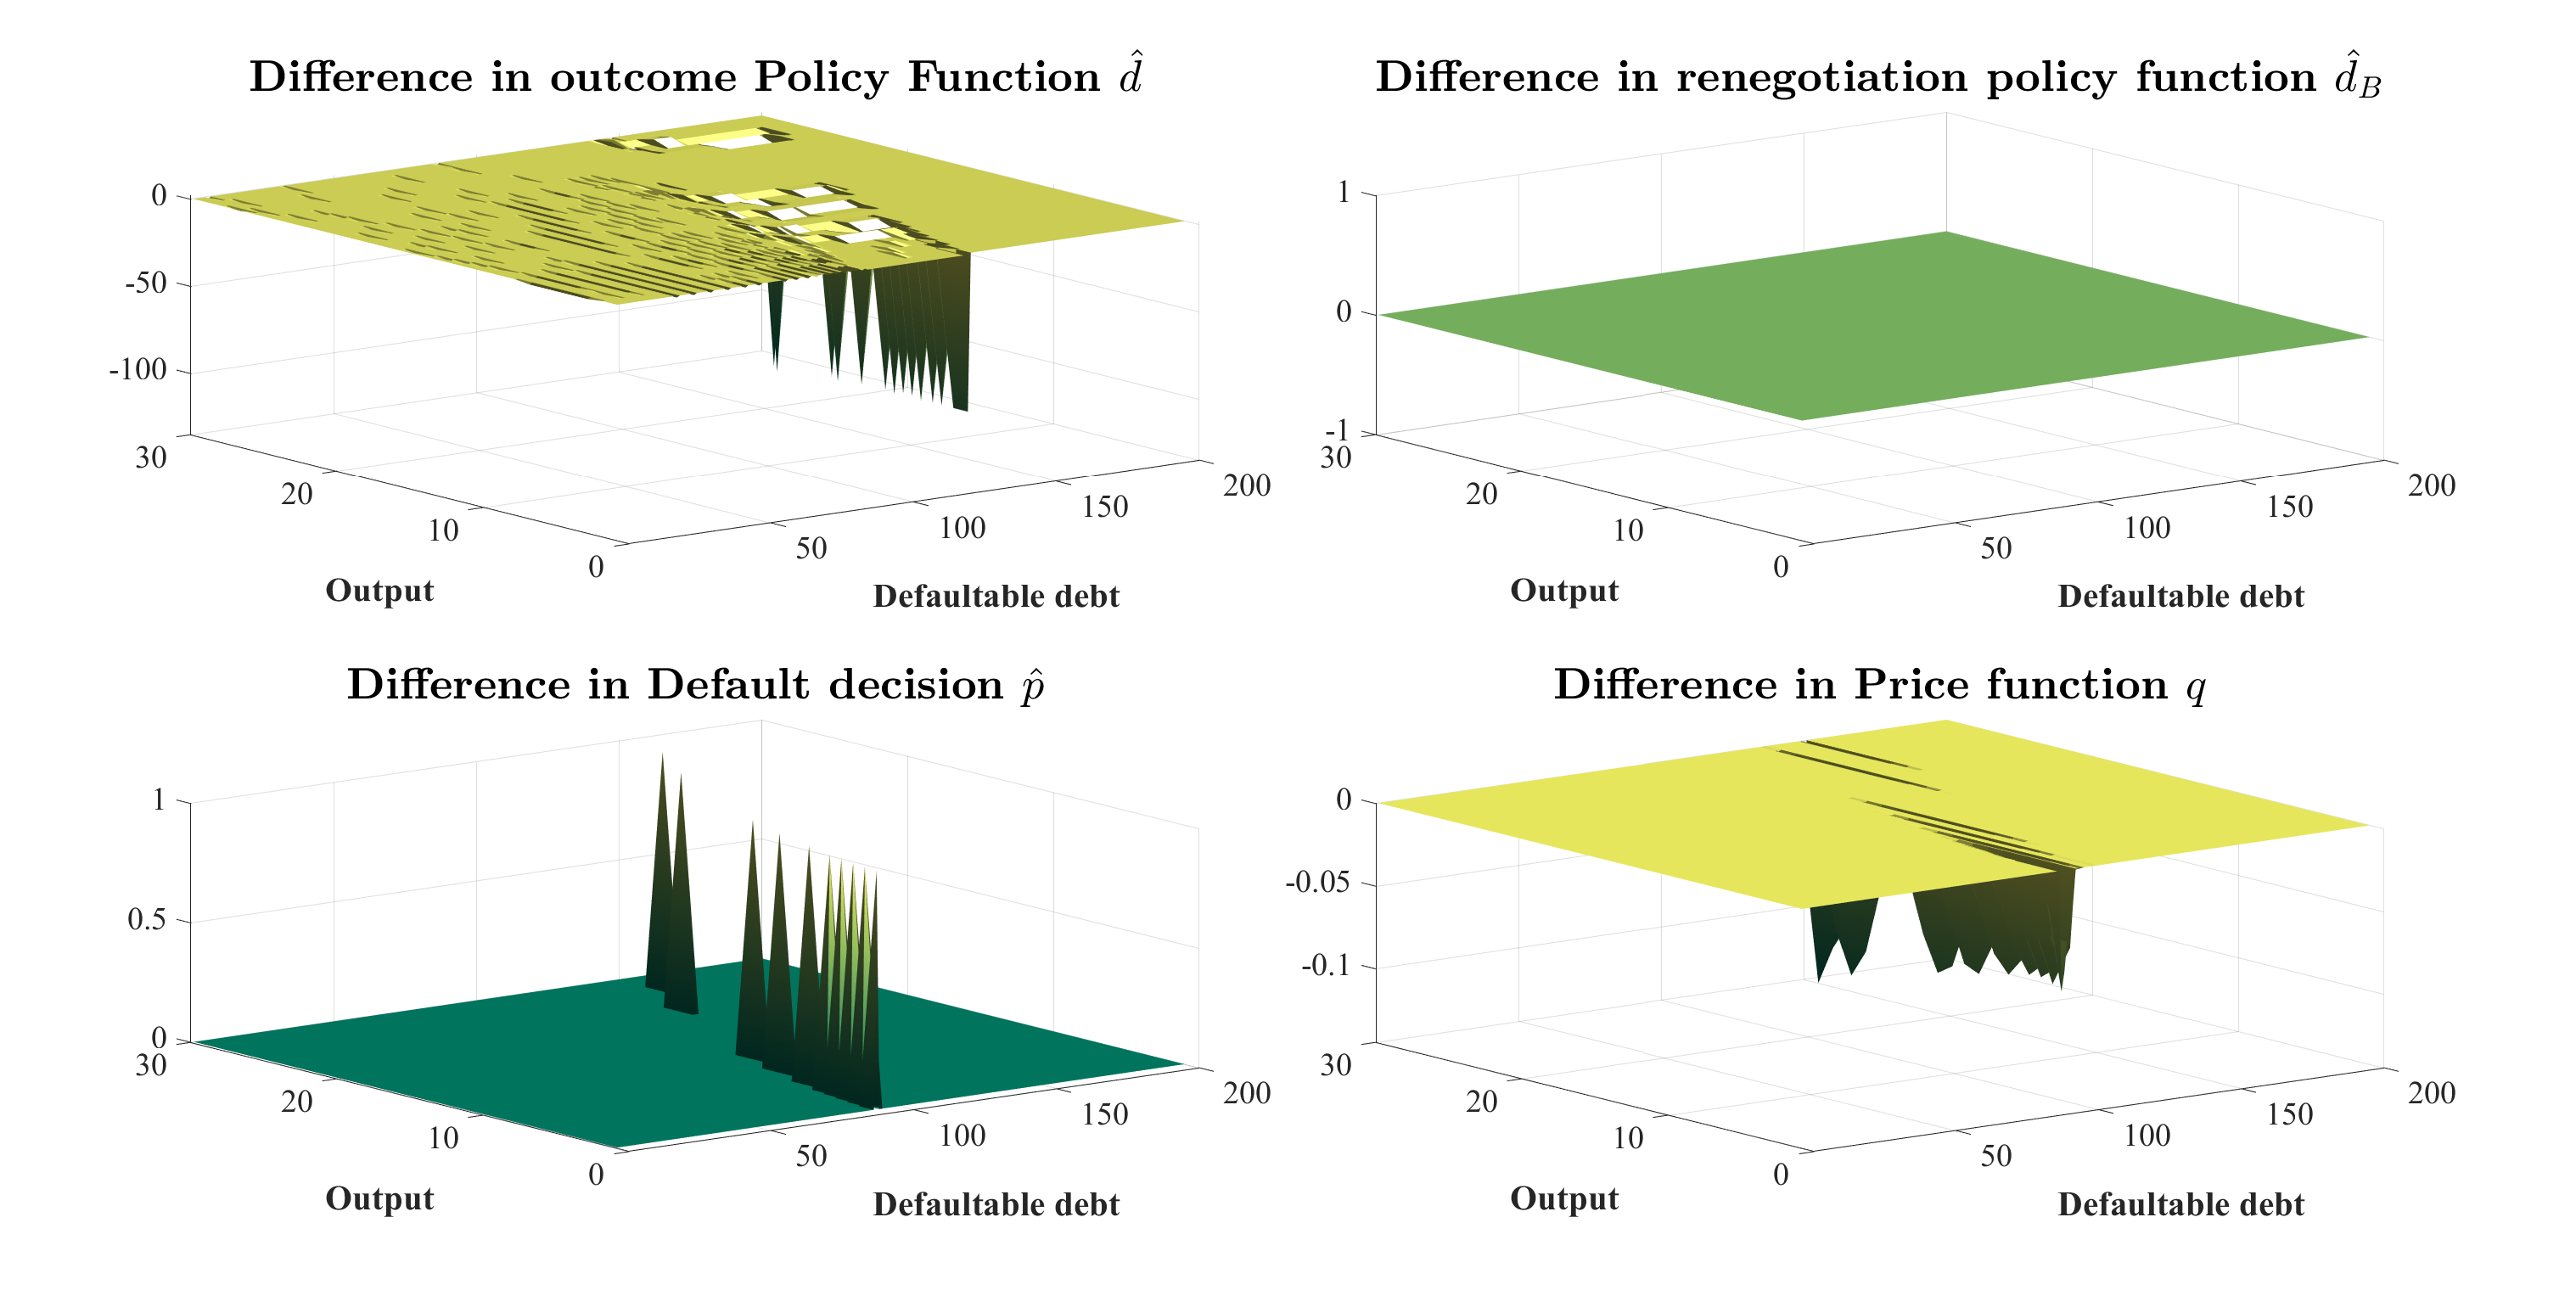
\includegraphics[scale=0.32]{FigureMult_NO.eps}
   }
       \begin{tablenotes}
      \footnotesize
      \item Figure 3.6 presents the differences in policy functions $\hat{d}$, $\hat{d}_B$, default decision $\hat{p}$ and price function $q$ between the "good" equilibrium and "bad" equilibrium starting position. 
    \end{tablenotes}
\end{figure}
%%%%%%%%%%%%%%%%%%%%%%%%%%%%%%%%%%%%%%%%%%%%%%%%%%%%%%%%%%
%%%%%%%%%%%%%%%%%%%%%%%%%%%%%%%%%%%%%%%%%%%%%%%%%%%%%%%%%%
\begin{figure}[H] \label{fig:mult eurobond}
 \caption{\textbf{Differences in Policy and Price functions (Eurobonds)}}
 \resizebox{\columnwidth}{!}{%
   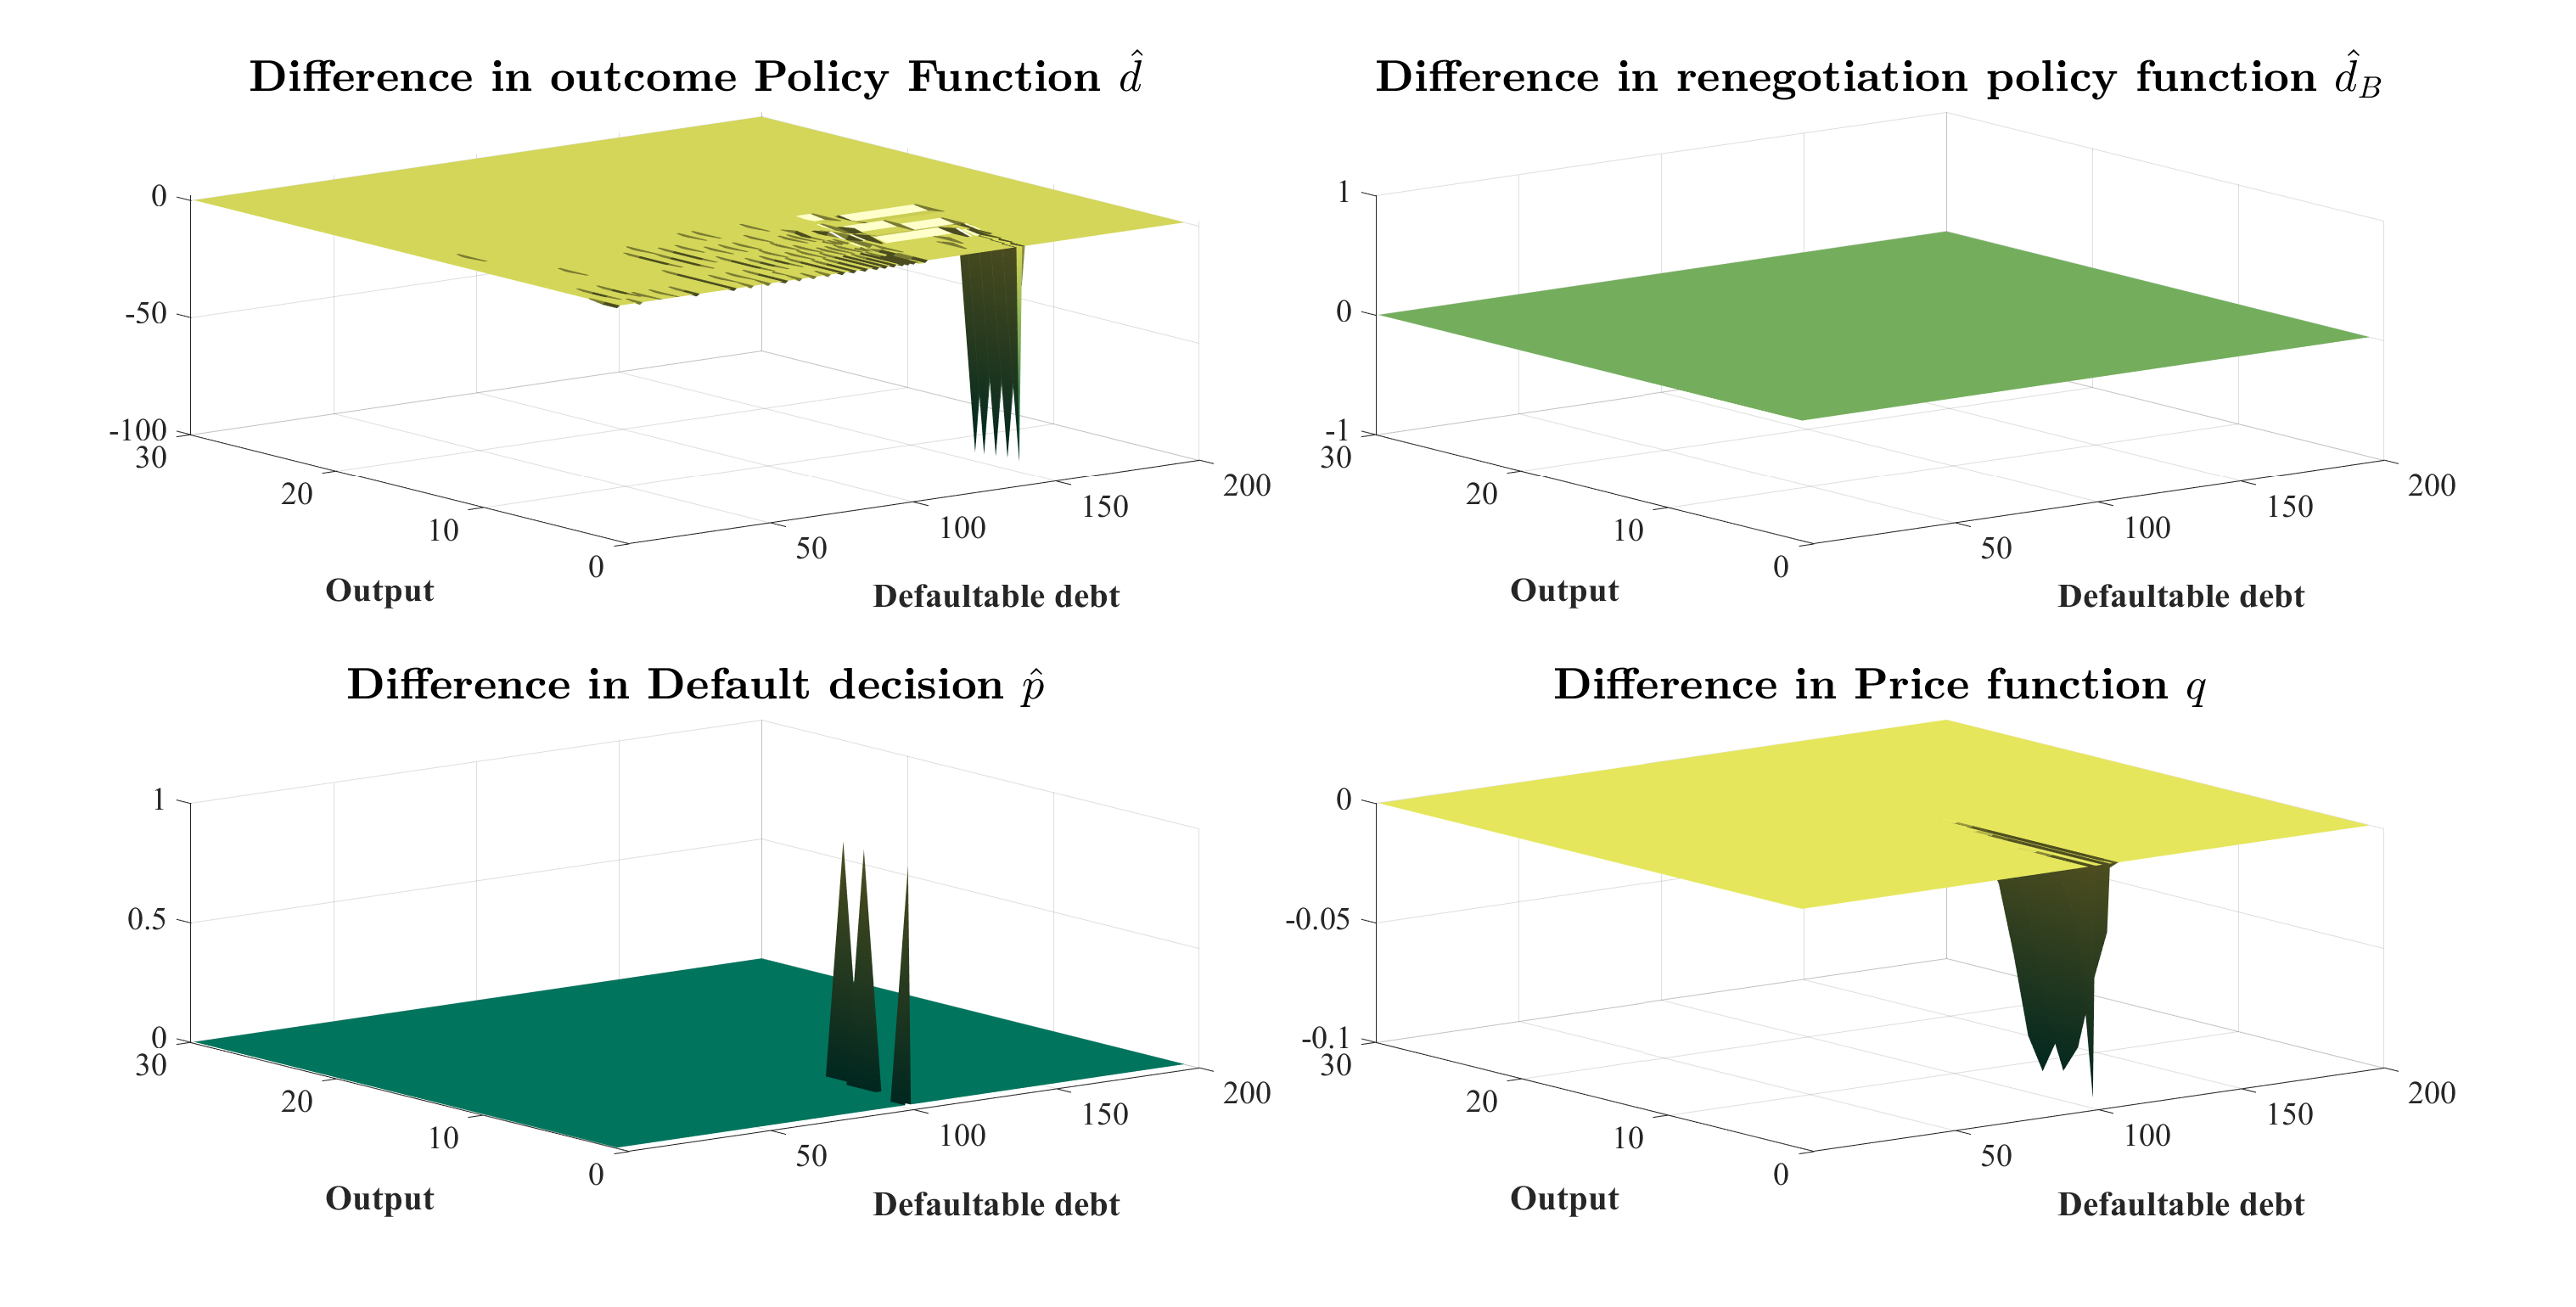
\includegraphics[scale=0.32]{FigureMult_YES.eps}
   }
       \begin{tablenotes}
      \footnotesize
      \item Figure 3.7 presents the differences in policy functions $\hat{d}$, $\hat{d}_B$, default decision $\hat{p}$ and price function $q$ between the "good" equilibrium and "bad" equilibrium starting position. Differences are calculated for each grid point. Only the grid points where $e = 0$ are shown.
    \end{tablenotes}
\end{figure}
%%%%%%%%%%%%%%%%%%%%%%%%%%%%%%%%%%%%%%%%%%%%%%%%%%%%%%%%%%